\documentclass[11pt,
% draft,
titlepage,oneside]{book}

%%%%%%%%%%%%%%%%%%%%%%%%%%%%%%%%%%%%%%%%%%%%%%%%%%%%%%%%%%%%%%%%%%%%%%%%%%%%%%%%%%%%%%%%%%%%%%
%   DO NOT MODIFY THESE LINES
%
%
%   Here is the header file that will set all the spacing to be correct and include the basic packages.
%   The second include here is a header file where you should put your include packages and your
%   user-defined commands.



%%%%%%%%%%%%%%%%%%%%%%%%%%%%%%%%%%%%%%%%%%%%%%%%%%%%%%%%%%%%%%%%%%%%%%%%%%%%%%%%%%%%%%%%%%%%%%
%
%   DO NOT MODIFY THIS FILE UNLESS ABSOLUTELY NECESSARY!!!!!
%
%%%%%%%%%%%%%%%%%%%%%%%%%%%%%%%%%%%%%%%%%%%%%%%%%%%%%%%%%%%%%%%%%%%%%%%%%%%%%%%%%%%%%%%%%%%%%%



\usepackage{layout}
%\usepackage{amsmath, amsthm}  These shouldn't be necessary for 'All' documents. Also amsrefs conflicts with natbib
%\usepackage{amssymb, amsrefs} You can add these in your custom header
\usepackage{graphicx}
\usepackage{setspace}
\usepackage{textcomp}
\usepackage[a]{esvect}
\usepackage[letterpaper]{geometry}


%   The following commands allow you to use each of these mathematical terms as theorem environments.
%\newtheorem{theorem}{Theorem}[section]
%\newtheorem{lemma}[theorem]{Lemma}
%\newtheorem{proposition}[theorem]{Proposition}
%\newtheorem{corollary}[theorem]{Corollary}
%\newtheorem{definition}[theorem]{Definition}
%\newtheorem{conjecture}[theorem]{Conjecture}
%\newtheorem{ex}[theorem]{Example}

%\DeclareGraphicsRule{.tif}{png}{.png}{`convert #1 `dirname #1`/`basename #1 .tif`.png}  Auto convert .tif files... I don't need this. 

\setlength{\hoffset}{0in} \setlength{\voffset}{0in}
\setlength{\oddsidemargin}{.5in} \setlength{\evensidemargin}{0in}
\setlength{\topmargin}{-0.15in} \setlength{\textwidth}{6.15in}
\setlength{\textheight}{614pt} \setlength{\marginparwidth}{64pt}
\setlength{\marginparsep}{8pt}

\headheight 12pt                    % included in the documentclass declaration before you print
\headsep 0.2in                      % a final version.  This will place a black mark next to any
\parskip 0.2in                      % line that LaTeX was forced to run into the right margin, so
\parindent 0.0in                    % you can more easily spot and fix this problem.

%   Your header stuff goes here
\usepackage{natbib}
\usepackage{amsmath}
\usepackage{amsthm}
\usepackage{amssymb}
\usepackage{hyperref}
\usepackage{cleveref}
\usepackage[framed]{mcode}
\usepackage{tikz}
\usepackage{units}

\usetikzlibrary{matrix}
\usetikzlibrary{shapes.geometric}
\usetikzlibrary{shapes.misc}
\usetikzlibrary{decorations.pathmorphing}
\usetikzlibrary{arrows}
\usetikzlibrary{backgrounds}
\usetikzlibrary{positioning}
\usetikzlibrary{fadings}
\DeclareMathOperator*{\argmin}{arg\,min}
\DeclareMathOperator*{\supp}{supp}
\DeclareMathOperator*{\acos}{acos}

\theoremstyle{plain}
\newtheorem{thm}{Theorem}[section]
\newtheorem{lem}[thm]{Lemma}
\newtheorem{prop}[thm]{Proposition}
\newtheorem{cor}[thm]{Corollary}
\newtheorem{defn}[thm]{Definition}

\renewcommand{\bar}{\overline}
\renewcommand{\hat}{\widehat}
\renewcommand{\tilde}{\widetilde}
\newcommand{\eqdef}{\stackrel{\rm def}{=}}
\newcommand{\eps}{\varepsilon}
\newcommand{\del}{\partial}
\newcommand{\RR}{\ensuremath{\mathbb R}}
\newcommand{\vect}[1]{\boldsymbol{#1}}
\newcommand{\DD}{\ensuremath{\mathfrak D}}
\newcommand{\K}{\ensuremath{\mathscr K}}
\newcommand{\R}{\ensuremath{\mathscr R}}
\newcommand{\HH}{\ensuremath{\mathscr H}}


%
%
%   This include must come after all of your other header stuff...that is why it's here
%   and not in the header file.
\usepackage{fancyhdr}
%   This sets the page header style for the preliminary pages.  It gets reset for the chapters.
\pagestyle{fancy} \fancyhf{}
\renewcommand{\headrulewidth}{0pt}
\cfoot[\fancyplain{}{\thepage}]{\fancyplain{}{\thepage}}
\lhead[\fancyplain{}{\leftmark}]{}
%
%   Now we actually begin the document
\begin{document}
%   This is your title page.  The changes here should be obvious.

\begin{titlepage}

\begin{center}
    \Large POINT SPREAD FUNCTION ESTIMATION AND UNCERTAINTY QUANTIFICATION\\ 
	\vspace{.5cm}
    \normalsize By\\
    \vspace{.5cm}
      Kevin Thomas Joyce\\
    \vspace{.5cm}
      B.S., Montana State University, Bozeman, MT, 2006\\ 
      M.S., Montana State University, Bozeman, MT, 2009\\   
    \vspace{.5cm}
	Dissertation\\
	\vspace{.5cm}
    presented in partial fulfillment of the requirements\\
    for the degree of\\
    \vspace{.5cm}
    Doctorate of Philosophy\\
	in Mathematics\\
    \vspace{.5cm}
    The University of Montana\\
	Missoula, MT\\
    \vspace{.5cm}
    May 2016\\
	\vspace{.5cm}
	Approved by:\\
	\vspace{.5cm}
	Sandy Ross, Associate Dean of the Graduate School\\  
	Graduate School\\
	\vspace{.5cm}
	Dr. Johnathan Bardsley, Co-Chair\\  
	Mathematical Sciences\\
	\vspace{.5cm}
	Dr. Aaron Luttman, Co-Chair\\  
	Signals Processing and Applied Mathematics\\
	National Security Technologies, LLC, Las Vegas, NV\\
	\vspace{.5cm}
	Dr. Jon Graham\\  
	Mathematical Sciences\\
	\vspace{.5cm}
	Dr. Peter Golubtsov\\  
        Department of Physics\\
        Lomonosov Moscow State University\\
	\vspace{.5cm}
	Dr. Leonid Kalachev\\  
	Mathematical Sciences\\
\end{center}

\vspace{1.25in}


\pagebreak

\end{titlepage}

\singlespacing \addcontentsline{toc}{chapter}{Abstract}
%
%   This begins the abstract page
%
\pagenumbering{roman}                   % Setting the page numbering to begin with lowercase
\setcounter{page}{2}                    % roman numeral 2.
%
%   The first line is your name, followed by degree and completion month/year as above.
%

Joyce, Kevin, Doctorate of Philosophy, May 2016 \hfill Mathematics
   
% Self Explanatory (but not all caps as on the title page)
Point Spread Function Estimation and Uncertainty Quantification

%
Committee Chairs: Johnathan Bardsley, Ph.D.~and Aaron Luttman, Ph.D.    % Self Explanatory
%
\setlength{\parindent}{2ex}
%
% Now for you abstract text:
%


\indent 
An important component of analyzing images quantitatively is modeling image blur due to effects from the system for image capture. 
When the effect of image blur is assumed to be translation invariant and isotropic, it can be generally modeled as convolution with a radially symmetric kernel, called the point spread function (PSF).
Standard techniques for estimating the PSF involve imaging a bright point source, but this is not always feasible (e.g.~high energy radiography).  
This work provides a novel non-parametric approach to estimating the PSF from a calibration image of a vertical edge.
Moreover, the approach is within a hierarchical Bayesian framework that in addition to providing a method for estimation, also gives a quantification of uncertainty in the estimate by Markov Chain Monte Carlo (MCMC) methods.
%This work takes a novel non-parametric approach to modeling a radially symmetric PSF, in which an estimate can be obtained from the calibration image of a vertical edge.

\indent
In the development, we employ a recently developed enhancement to Gibbs sampling, referred to as partial collapse. 
The improved algorithm has been independently derived in several other works, however, it has been shown that partial collapse may be improperly implemented resulting in a sampling algorithm that that no longer converges to the desired posterior.
The algorithm we present is proven to satisfy invariance with respect to the target density.
This work and its implementation on radiographic data from the U.S.~Department of Energy's Cygnus high-energy X-ray diagnostic system have culminated in a paper titled ``Partially Collapsed Gibbs Samplers for Linear Inverse Problems and Applications to X-ray Imaging,'' which is under review for a special issue of journal \emph{Inverse Problems}.

\indent
The other component of this work is mainly theoretical and attempts to develop from first principles the requisite functional analysis to make the integration based model derived in the first chapter rigorous.
The literature source is from functional analysis related to distribution theory for linear partial differential equations, and briefly addresses infinite dimensional probability theory for Hilbert space-valued stochastic processes, a burgeoning and very active research area for the analysis of inverse problems.
To our knowledge, this provides a new development of a notion of radial symmetry for $L^2$ based distributions.
This work results in defining an $L^2$ complete space of radially symmetric distributions, which is an important step toward rigorously placing the PSF estimation problem in the infinite dimensional framework and is part of ongoing work toward that end.

\pagebreak

\setlength{\parindent}{0.0in}
%
%%%%%%%%%%%%%%%%%%%%%%%%%%%%%%%%%%%%%%%%%%%%%%%%%%%%%%%%%%%%%%%%%%%%%%%%%%%%%%%%%%%%%%%%%%%%%%%


%   The next two lines may be deleted if you do not have acknowledgements.
\addcontentsline{toc}{chapter}{Acknowledgments}
../AcknowledgmentsPage.tex


% The next two lines may be deleted if you do not have a notations page.
\onehalfspacing \addcontentsline{toc}{chapter}{Notations}
%   This is the file for your notations page.  Do not modify the next line.
{\bf {\Large Notations}} \\
%   Put your notations here

% Image Model
{\bf {\large Image Model}}\\
$p \dotfill$ Point spread function\\
$b \dotfill$ Observed data\\
$\G \dotfill$ Forward edge-blur operator on a radial profile\\

% Sets 
{\bf {\large Sets}}\\
$\Z$\dotfill Integers\\
$\R$\dotfill Real numbers\\
$\R^k$  \dotfill $k$-dimensional vector space over real numbers\\
$\rem xi$\dotfill The vector $(x_1,\dots,x_{i-1},x_{i+1},\dots,x_k)$\\

% Functional Analysis
{\bf {\large Functional Analysis}}\\
$\HH \dotfill$ Hilbert space\\
$\|\cdot \| \dotfill$ Norm\\
$\langle \cdot,\cdot \rangle \dotfill$ Inner product\\
$\mathscr X^*$\dotfill Dual space of $\mathscr X$\\
$\DD$\dotfill Compactly supported smooth test functions\\
$\DD^*$\dotfill Space of distributions\\
$\KK$\dotfill Space of radially symmetric functions\\
$\PP$\dotfill Space of radial profiles\\
$\argmin_{x\in A} \Phi(x) \dotfill$ The $x\in A$ such that $\Phi(x)$ is minimized\\
$\|\cdot \|_{TV} \dotfill$ Total variation norm\\

% Probability
{\bf {\large Probability}}\\
%$\Omega \dotfill$ Set of outcomes\\
%$\mathcal F \dotfill$ Sigma-algebra of events\\
%$\sigma(\tau) \dotfill$ Sigma-algebra generated by the set $\tau$\\
%$\mathcal{B}(\R^k) \dotfill$ Borel sets on $\R^k$\\
$\mathbb{P} \dotfill$ Probabilty measure\\
$\mathbb{E} \dotfill$ Probabilty expectation\\
$K \dotfill$ Transition kernel\\
$\K \dotfill$ Transition operator\\
$\pi(\cdot) \dotfill$ Probability density\\
$\pi(\cdot|\cdot) \dotfill$ Conditional probability density\\
$X\sim \pi \dotfill$ Random variable $X$ has distribution $p$ \\


% Handy help for stacking words, using braces
% $\overbrace{\hbox{Text}}^{\hbox{text above}}$
% $\underbrace{\hbox{Text}}_{\hbox{text below}}$
% $\stackrel{\hbox{Text above}}{\hbox{Text below}}$
\pagebreak



%%%%%%%%%%%%%%%%%%%%%%%%%%%%%%%%%%%%%%%%%%%%%%%%%%%%%%%%%%%%%%%%%%%%%%%%%%%%%%%%%%%%%%%%%%%%%
%
%   DO NOT MODIFY THESE LINES
%
% Automatically generates a table of contents, separated by page breaks
\onehalfspacing \rhead{} \tableofcontents \pagebreak
%
%%%%%%%%%%%%%%%%%%%%%%%%%%%%%%%%%%%%%%%%%%%%%%%%%%%%%%%%%%%%%%%%%%%%%%%%%%%%%%%%%%%%%%%%%%%%%





%   Generates a list of tables.  Delete the next two lines if you do not want a list of tables.
%   Note that you should have such a list if you have more than one table.
\addcontentsline{toc}{chapter}{List of Tables} \listoftables
\pagebreak


%   Generates a list of figures.  Delete the next two lines if you do not want a list of figures,
%   but, as with tables, you should have such a list if you have more than one figure.
\addcontentsline{toc}{chapter}{List of Figures} \listoffigures
\pagebreak

%   Generates a list of algorithms.  Delete the next two lines if you do not want a list of algorithms,
%   but, as with tables, you should have such a list if you have more than one algorithm.
\addcontentsline{toc}{chapter}{List of Algorithms} \listofalgorithms
\pagebreak


%%%%%%%%%%%%%%%%%%%%%%%%%%%%%%%%%%%%%%%%%%%%%%%%%%%%%%%%%%%%%%%%%%%%%%%%%%%%%%%%%%%%%%%%%%%%%%%
%   DO NOT MODIFY THESE LINES
%
%   Restart the page numbering with arabic numbering starting at 1
\pagenumbering{arabic} \setcounter{page}{1}
%
%%%%%%%%%%%%%%%%%%%%%%%%%%%%%%%%%%%%%%%%%%%%%%%%%%%%%%%%%%%%%%%%%%%%%%%%%%%%%%%%%%%%%%%%%%%%%%%


%   Now reset the spacing for the chapters.  Spacing can be 1.5 or 2, but double is recommended.
%\onehalfspacing
\doublespacing




%%%%%%%%%%%%%%%%%%%%%%%%%%%%%%%%%%%%%%%%%%%%%%%%%%%%%%%%%%%%%%%%%%%%%%%%%%%%%%%%%%%%%%%%%%%%%%%%
%
%   DO NOT MODIFY THESE LINES
%   Here we reset the header style for the chapters.
\pagestyle{headings}
%
%%%%%%%%%%%%%%%%%%%%%%%%%%%%%%%%%%%%%%%%%%%%%%%%%%%%%%%%%%%%%%%%%%%%%%%%%%%%%%%%%%%%%%%%%%%%%%%%%
%
%                              CHAPTERS
%


%   Here you include your chapter files - see chapter1.tex for format
\setlength{\parindent}{2ex}
\begin{chapter}{Introduction}\label{chapter:introduction}
  In addition to being a rich source of artistic and creative inspiration, pictures, or more precicely visual data, have been a crucial source of scientific information.
  Even the word ``observation'' generally connotes close visual scrutiny, and its use as a catch-all for the measured verification of a hypothesis exemplifies the central role of visual perception in science.
  Many important scientific results have used visual data to discover and explain natural phenomena; for example, visual observations such as the color and shape of various plant organs in Gregor Mendel's famous experiments on hybridized peas formed the primary source of data for developing his famous model for genetic inheritance \citep{mendel????}.
  Arthur Eddington's famous celestial observations in the early 20th century, which provided the first experimental evidence supporting Albert Einstein's general theory of relativity, recorded the gravitationally lensed path of a comet on photographs taken during a solar eclipse \citep{eddington1902}.
%  The richness of the raw data content in an image and our human propensity to digest visual information -- the focus of our mind's eye, so to say -- make visual data in images a compelling source of scientific evidence and information.
  Yet, in these cases, only the \emph{qualitative} components of the visual response and their relationship to the experiment were relevant.
  With the advent of the camera, photosensitive chemistry, and later digital imaging technology, high-fidelity recording of visual observations became possible, allowing the potential to \emph{quantitatively} analyze visual information.
  The ever-progressing technology in optical science and engineering are rapidly increasing the amount of data that can be measured in an image; yet, the extreme quantity and spatial organization that comes with high resolution data makes a rigorous quantitative analysis challenging.

  Images, when viewed quantitatively, can be described as the response of the incidence of light, and the subsequent exchange of energy, on a grid of regularly spaced points, which we refer to as pixels.
  The domain of interest for imaging systems can vary greatly in both spatial dimension and the spectrum of light captured. 
  The energy response of light is spectrum dependent, and typically is analyzed at fixed bands of frequency with very high spatial resolution.
%  The raw volume of recorded data is usually very large.
  For example, astronomical images captured by the interstellar robotic probes Voyagers I and II measured 5 spectral bands in the visible spetrum on a pixel grid with dimension $800 \times 800$ \citep{voyager}.
  In medical imaging, computed tomography (CT) is an imaging process where a series of axial measurements of attenuation of electromagnetic radiation are used to reconstruct a cross-section of a scanned object \citep{epstein2008}.
  Of primary focus in this work are pulsed X-ray measurements, referred to as radiographs, that are used as an experimental diagnostic of high-energy physics experiments.  
  In this case, X-rays are pulsed through an experiment, then the attenuated X-rays excite a crystal that responds by luminescing visible light at an intensity related directly to the energy of the attenuated wave-front.  
  The light is then measured on a high resolution array (on the order of $1000\times1000$ or more) of carge coupled devices (CCD) calibrated to count photons at a specified spectral band.

  We have established the form that image data usually takes -- \emph{what} the data is. 
  Now, \emph{how} does one analyze it?
  Although images often provide a large volume of data, their spatial nature make measurements at each pixel highly dependent on measurments of adjacent pixels.
  A quantitative analysis of the image cannot assume that measured values are independent.
  But it is precisely this lack of independence that makes an image interesting -- independent image data is ``gray noise'' from which one can only infer the average of the measured pixels.
  %A quantitative analysis of image data must take into account pixel-to-pixel dependence.
  %That is, the measured values at one pixel depends heavily on adjacent or neighboring pixels, thus, one expects the measured data to be highly correlated.
  From a statistical point of view, the field of spatial statistics considers broadly the analysis of data that is structured and correlated in this way.
%  The relatively recent date of this publication (in mathematical terms) coupled with the prevalence of image data prior to this, hints that the requisite tools for a rigorous statistical analysis require modern mathematical theory and state of the art computation.
  This field has had much development over the past half-century and has inspired a wealth of theory and computational tools, but is far from complete.
  Moreover, a broad field of scientific disciplines have considered image data, or more generally spatially correlated data, in one way or another; fields such as astronomy, astrophysics, biology, medicine, geology, computer science, and nuclear physics to name a few.
  The book \citep{cressie1993statistics} provides an excellent overview of the history and current methods for statistical methods for spatial data.
%  Each have a unique perspective on the problem, and a vast literature on the subject has accumulated.
  Although much work has been done, it is still a very active research area and is far from the level of consensus and understanding that analysis of independently sampled data has achieved. 
  The aim of this work is to develop and adapt current models and methods for estimation and quantifying uncertainty to a small component of image analysis related specifically to the \emph{system for capturing images}.
  Understanding this component is an important preliminary step to developing methods for quantitatively analyzing the images themselves.

\section{Modeling blur with a PSF}
  
  One major component of the spatial relationship of neighboring pixels of an image is due to blur from the imaging instrumentation.
  That is, under the assumption that arbitrary images are measured by a consistently modeled system, what contribution does this system have on how pixels are related, and how can we quantify this relationship?
  A widely used model for blurring \citep{hansen2010,jain1989,vogel2002,epstein2008} expresses this relationship through a point-wise integral product with a function that describes interaction with neighboring points, e.g.
  \begin{equation}\label{eq:generalPsf}
    b(x,y) = \iint_{\Omega} k(x,y;s,t) f(s,t)\,dsdt
  \end{equation}
  where $b(x,y)$ represents the intensity of the blurred image at $(x,y)$; $f(s,t)$ represents the intensity of the ideal un-blurred image at $(s,t)$ in $\Omega$; and $k$ is a function that describes the blur for each $(x,y)$.
  Informally, integration against the function $k(x,y;\cdot,\cdot)$ represents the ``spread'' of blurred pixel at $(x,y)$, hence, is referred to as a point spread function (PSF).
  The form of $k$ is guided by optical principles and the physics of the system that generally dictate that, for fixed $(x,y)$, $k(x,y;\cdot,\cdot)$ is concentrated (in the measured or integrated sense) at $(x,y)$ and continuously decays as the distance from $(s,t)$ to $(x,y)$ increases.
  The function in \eqref{eq:generalPsf} is often interpreted as a family of PSFs $k(x,y;\cdot,\cdot)$ indexed at each $(x,y)$.

  Under the additional assumption that the effect of blur is spatially invariant in $(x,y)$ (that is, invariant to translations of $(x,y)$), then $k(x,y;s,t)$ can be expressed by translating some function $\tilde k(s,t)$ to $(x,y)$; i.e.~ $k(x,y;s,t) = \tilde k(x-s,y-t)$.  
  Dropping the tilde notation, we have
\begin{equation}\label{eq:convolutionDeterministic}
  b(x,y) = \iint_{\Omega} k(x-s,y-t) f(s,t)\,dsdt.
\end{equation}
  The integral product in \eqref{eq:generalPsf} is called the convolution of $f$ by $k$.
  The assumptions for modeling blur in this form are quite common, and methods that estimate $f$ from $b$ given $k$ are referred to as deconvolution techniques.
  Note that a change of variables by $s'=x-s$ and $t'=y-t$ results in a convolution of $k$ by $f$, which is to say that convolution, as an operation, is symmetric.
  This dual relationship between the PSF and the image will allow us to use the framework and tools of deconvolution for the problem of PSF estimation.
  That is
  \begin{equation}\label{eq:dualConvolutionDeterministic}
    b(x,y) = \iint_{\Omega} k(s,t) f(x-s,y-t)\,dsdt.
  \end{equation}

  Typically, deconvolution methods assume that the form of the PSF can be accurately described by modeling the imaging system \citep{jain1989,hansen2006}, but for complex imaging systems such as the one described for X-ray radiography, this is not realistic.
  Instead, if the imaging system is designed so that repeated images can be taken under consistent conditions, then by convolution symmetry in \eqref{eq:dualConvolutionDeterministic}, the blurring of a \emph{known calibration image} can be cast as deconvolving the PSF from the ideal $f$ corresponding to the known image.

  Recall that the PSF models the blurring response of a single point.
  So, a direct estimate of $k$ can be obtained by imaging a bright point source, which approximates the impulse response to \eqref{eq:dualConvolutionDeterministic}.
  In astronomical imaging, the point source can be a bright distant star, or in a controlled setting where visible light is measured, a focused laser beam provides a good point source estimate.
  However, in the spectral regime of high-frequency X-rays, the problem of focusing high frequency-light is notoriously difficult and usually is impractical in situations of interest, so a point source estimate of the PSF is usually unavailable at these frequencies.
  Instead, the system response of a uniformly opaque calibration object with a simple geometry can be measured.
  Under the assumption that the object is sufficiently thick so that it attenuates X-rays sufficiently so that the ideal image is given by an indicator function for a known set $E \subseteq \Omega$, one can form a deconvolution problem that exploits our control over the geometry of $E$.
  Calibration objects typically have simple geometry and reduce the complexity of solving \eqref{eq:dualConvolutionDeterministic}.
  When the calibration object is a vertical edge at a known and fixed location in the imaging plane, then $E$ is the half plane, and its characteristic function depends only on $s$ and is given by $f(s) = 1$ if $s\ge0$ and $f(s)=0$ if $s <0$. 
  The model for blur in \ref{eq:convolutionDeterministic} reduces to
\begin{equation}\label{eq:psfForwardModelDeterministic}
  b(x) = \iint_{\Omega} k(s,t) f_E(x-s)dsdt. 
\end{equation}
  Note that $b$ no longer depends on $y$, hence the model output provides data only in the horizontal dimension.
  This leads to the problem of estimating $k$ from $b$ in \eqref{eq:psfForwardModelDeterministic} being underdetermined, since there are generally many distinct $k$ that can result in the same output $b$.
  An additional assumption of \emph{radial symmetry} on $k$ will sufficiently constrain the problem and is addressed in the following section.

\section{The Abel transform and a deterministic solution}
  In this section we show that radial symmetry is sufficient to guarantee a unique analytic answer.
  This will lay out an analytic solution to \eqref{eq:psfForwardModelDeterministic}, however, it will be inadequate as we will see in the following section.

  A large part of designing a system for imaging is to minimize the effect of blur.
  Often, limitations due to physical laws put a lower bound on the measurement precision so that even an optimal design cannot ignore the effect of blur.
  Although arbitrary resolution may be impossible, engineering effort can still optimize accuracy, or, equivalently, minimize bias.
  Hence, an optimally designed imaging system should exhibit isotropic blur (an absence of direction bias), so that, in the convolution model, the PSF is radially symmetric.
  In fact, many parametrically modeled PSFs assume radially symmetry \citep{doering1992,jain1989,kundur1996blind,watson1993}.  

  When one assumes that the PSF of their system is radially symmetric, then it has a unique one-dimensional representation.
  That is, there exists a function $p$ defined on $\Omega_1 \subseteq (0,\infty)$ so that $k(s,t) = p\left(\sqrt{s^2 + t^2}\right)$.  
  The function $p$ is referred to as the radial profile of $k$.
  When $\Omega$ is almost all of $\RR^2$ (in the sense of measure), then substituting $p$ into \eqref{eq:psfForwardModelDeterministic} gives
  \begin{align}
    b(x) &= \int_{-\infty}^x \left(\int_{-\infty}^\infty p\left(\sqrt{s^2 + t^2}\right)\,dt\right)ds \nonumber \\
         &\eqdef \int_{-\infty}^x \ell(s)ds. \label{eq:abelForward}
  \end{align}
  The function $\ell(s)$ is the integration along a line perpendicular to the edge $E$, and its form is commonly encountered in tomographic imaging science.

  Observe that $b$ exhibits point symmetry about $b(0)$.
  To see this analytically, for $x>0$ the formulation in terms of the Abel transform in \eqref{eq:abelForward} gives
  \begin{align}
    b(x) &= \int_{-\infty}^0 \ell(s)ds + \int_0^x \ell(s)ds \nonumber \\
         &= b(0) - \int_0^{-x}\ell(s')ds'  \nonumber \\
         &= b(0) - b(-x).
  \end{align}

%  The collection of line integrals parametrized by their angle of incidence is called the Radon transform of $k$, and when $k$ is radially symmetric, the transform is completely determined by a single projection.
  The operator that takes the radial profile $p$ to $l$ is called the Abel transform and is encountered in tomographic imaging.
  In \citep{epstein2008}, the following explicit expression for obtaining $p$, given $\ell$ is derived;
  \begin{equation} \label{eq:inverseAbel}
    p(r) = -\frac{1}{\pi r} \frac{d}{dr}\left(\int_r^\infty \frac{\ell(s) s ds}{ (s^2 - r^2)^{1/2} } \right).  
  \end{equation} 
  The following argument summarizes the arguments in \citep{epstein2008} to verify \eqref{eq:inverseAbel}.
  We can express the inner integral in \eqref{eq:abelForward} as
  \begin{equation}
    \ell(s) = 2\int_{|s|}^\infty \frac{p(t) t}{(t^2 - s^2)^{1/2}}\,dt \label{eq:abelForward2}
  \end{equation}
  by symmetry of the integrand (it is even) and a change of variable by $r = s^2 + t^2$.
  Now, interchanging the order of integration in \eqref{eq:inverseAbel} results in
  \begin{align} 
    \left(\int_r^\infty \frac{\ell(s) s ds}{ (s^2 - r^2)^{1/2} } \right)  
    &= \int_r^\infty\int_s^\infty \frac{p(t) ts}{(s^2 - r^2)^{1/2}(t^2 - s^2)^{1/2}}\,dtds \nonumber\\
    &= \int_r^\infty p(t) t\int_r^t \frac{s}{(s^2 - r^2)^{1/2}(t^2 - s^2)^{1/2}}\,dsdt. \label{eq:inverseAbelderive1}
  \end{align} 
  Another change of variables by $s^2 = \tau t^2 + (1-\tau)r^2$ (note $s\ge0$)
 % , results in $2sds = (t^2 - r^2)d\tau$, 
  so that the inner integral in \eqref{eq:inverseAbelderive1} is
  \begin{equation}
    \int_r^t \frac{s}{(s^2 - r^2)^{1/2}(t^2 - s^2)^{1/2}}\,ds
    = \frac 12 \int_0^1 \frac {1}{\tau^{1/2}(1-\tau)^{1/2}}\,d\tau. \label{eq:gammaIntegral}
  \end{equation}
  Note that the resulting integral is independent of both $r$ and $t$, thus, is constant. To evaluate it, recall the Gamma function identity
  \begin{equation} 
    \frac{\Gamma(\alpha)\Gamma(\beta)}{\Gamma(\alpha + \beta)} = \int_0^1 \tau^{-\alpha}(1-\tau)^{\alpha -1}\,d\tau,
  \end{equation}
  from which the expression in \eqref{eq:gammaIntegral} reduces to $\pi/2$.
  Collecting these results and applying the fundamental theorem of calculus with the assumption that $\lim_{r\to\infty}p(r) = 0$, proves the identity in \eqref{eq:inverseAbel}.
  
  With this result, $p$ can be analytically recovered from $b$ in \eqref{eq:abelForward}. 
  That is, given $b(x)$, the fundamental theorem of calculus gives $\ell(s)$ by differentiating $b(x)$, then applying the inversion formula in \eqref{eq:inverseAbel} to $b'(x)$ gives the radial profile $p(r)$.
  Hence, the assumption of radial symmetry sufficiently constrains the problem to uniquely determine the PSF from an edge calibration object illustrated in \Cref{fig:edgeData}.

  In theory, we have outlined a solution to the problem, but there is one more component to the noise-free model that has not been addressed -- random effects due to measurement error -- for which a direct application of outlined method on measured data will fail spectacularly, due to the estimation problem being ``ill-posed'' which we address in the next section.

\section{PSF reconstruction as an ill-posed inverse problem}
  The measurements of the imaging system are generally not deterministic and are subject to measurement noise.
  Precisely modeling the stochastic effect of measurement error is system dependent and can be quite complicated.
  In the X-ray radiography example, uncertainty can enter into the system at the luminescing crystal response, at the counts of CCD array, or through the electrical transmission of the signal.
  In order to be broadly applicable, and appealing generally to various central-limit-theorem-like results in probability \citep{durrett2010probability}, we model the stochastic measurement effect in aggregate as an additive, independent Gaussian noise process with zero mean and unknown variance.  
  For now, this assumption can be viewed as a small perturbation from the model, but its form will be important for the inference techniques developed in subsequent chapters.
  %The complete description of the model from which the PSF will be estimated is
  %  \begin{equation}\label{eq:psfForwardModelStochastic} 
  %    b(x) = \iint_{\Omega} k(s,t) f(x-s)dsdt + \eps_x  
  %  \end{equation}
  %where each $\eps_x \sim N(0,\sigma^2)$ and independently (in $x$) for some unknown variance $\sigma^2$.  

  Estimating a quantity of interest, in our case $k$, from indirect and noisy measurements, $b$, with a model where an operator takes $k$ \emph{to} $b$ (referred to as the \emph{forward operator}) is called an inverse problem.  
  The problem is called well-posed when the forward operator is invertible, and the inversion is insensitive to small perturbations.
  These famous conditions were laid out by Jacques Hadamard in the early 20th century \citep{hadamard1902}, but a number of important applications have arisen (among those computational imaging) where these conditions are violated, enough to the extent that the term ``inverse problems'', as it refers to the mathematical research area, is exclusively devoted to solving these \emph{ill-posed} problems.
  In particular, most cases of interest %are when the measurement model results in data \emph{not} in the range of the model operator and 
  exhibit a model where the inverse of the forward operator is very sensitive to perturbations.

  The discussion thus far for PSF reconstruction has been somewhat informal, as we have not defined a space for the PSF or its radial representation, so we have not formally defined a model forward operator.
  Defining these spaces in detail is somewhat technical and will be addressed in in Chapter 2; however, assuming these spaces have been defined, we can illustrate that the problem of reconstructing the radial profile is ill-posed.

  Instead of using the variable transform that views forward model in \eqref{eq:psfForwardModelDeterministic}an iterated integrals involving the Abel transform in \label{eq:abelForward}; instead 
  a change of variables in\eqref{eq:psfForwardModelDeterministic} (again assuming $\Omega$ is full measure in $\RR^2$)  by $(s,t) = T(r,v) = (r\cos v,r\sin v)$, has $|dT(r,v)| = r$ and 
  \begin{align}
    b(x) &= \int_0^\infty p(r) \left( \int_{-\pi}^\pi f_E(x - r\cos v)dv \right)\,r dr\nonumber \\
         &= \int_0^\infty p(r) g(x,r) r dr, \label{eq:radialForwardModelDeterministic}
  \end{align}
where
\begin{equation} \label{eq:radialForwardKernel}
  g(x,r) \eqdef \left\{\begin{array}{lr}
    0 & x < - r\\
    2(\pi - \acos(x/r)) & |x| < r\\
    2\pi &  x> r
  \end{array}\right..  
\end{equation}
  To see that $g$ has this form, note that integrating $f_E(x-r\cos v)$ is the radian measure of the set $\{v\in(-\pi,\pi): r\cos v \le x\}$; see \Cref{fig:radialForwardKernel}.  

  There are three key observations to make.
  From this viewpoint, the forward model is now a one-dimensional integral equation on the radial profile, as opposed to the two-dimensional problem in \eqref{eq:psfForwardModelDeterministic}.
  Second note that $g(x,r)$ is continuous (although it has a discontinuity in its partial derivatives across $r=s$).
  Finally, recall that the graph of $b(x)$ exhibits reflection symmetry about $b(0)$.
  So, $b(x)$ defined on either $(-\infty,0]$ or $[0,\infty)$ completely determines $p$.

  With these observations, we can define $G: \mathcal H_1 \to \mathcal H_2$ is an operator between closed isometric subspaces of $L^2([0,\infty))$ that acts by the integral equation in \eqref{eq:radialForwardModelDeterministic}, then $G$ is a compact Hilbert-Schmidt operator since $g$ is continuous and $\mathcal H_1$ and $\mathcal H_2$ are seperable Hilbert spaces.
  Thus, the spectral theory for such operators implies that $G$ has a countable spectrum that has zero as a limit point, hence, the inverse is unbounded, which results in an ill-posed problem. 
  See one of many texts on functional analysis \citep{bachman1966,rudin1991} and \citep{tikhonov1963,vogel2002,morozov1993} for the analytic treatment of ill-posed problems.

  Solving ill-posed inverse problems requires \emph{regularization} of the unbounded inverse.
  Recall that the original formulation of the problem is cast in terms of deconvolution, and much of the literature of inverse problems is devoted to this subject.
  This work draws heavily from techniques for that purpose. 
  In particular, we will take a Bayesian approach to the inverse problem so that in addition to estimating $k$, uncertainties in the estimate can quantified by analysing the posterior distribution.
  These methods have been the subject of much recent research (see the books \citep{calvetti2007introduction,kaipo2005,stuart2010}), and the problem of PSF reconstruction fits neatly into that framework once the spaces $\mathcal H_1$ and $\mathcal H_2$ have been defined.

\begin{figure}
  \begin{center}
\begin{tikzpicture}
  \draw (0,-2.2) -- (0,2.2);
  \draw (-3,0) -- (3,0);
  \draw[dotted] (-2.5,-2.2) node[below]{\footnotesize$x<-r$} -- (-2.5,2.2);
  \draw[dotted] (2.5,-2.2) node[below]{\footnotesize$x>r$} -- (2.5,2.2);
  \draw[dotted] (-1,-2.2) node[below right]{\footnotesize$|x|\le r$} -- (-1,2.2);

  \draw (0,0) circle[radius=2];
  \draw[very thick,red,domain=120:240] plot ({2*cos(\x)},{2*sin(\x)});
  \draw (0,0) -- (-1,{sqrt(3)});
  \draw (.3,0) node[above right]{$v$} arc [radius=.3,start angle=0,end angle=120];
\end{tikzpicture}
  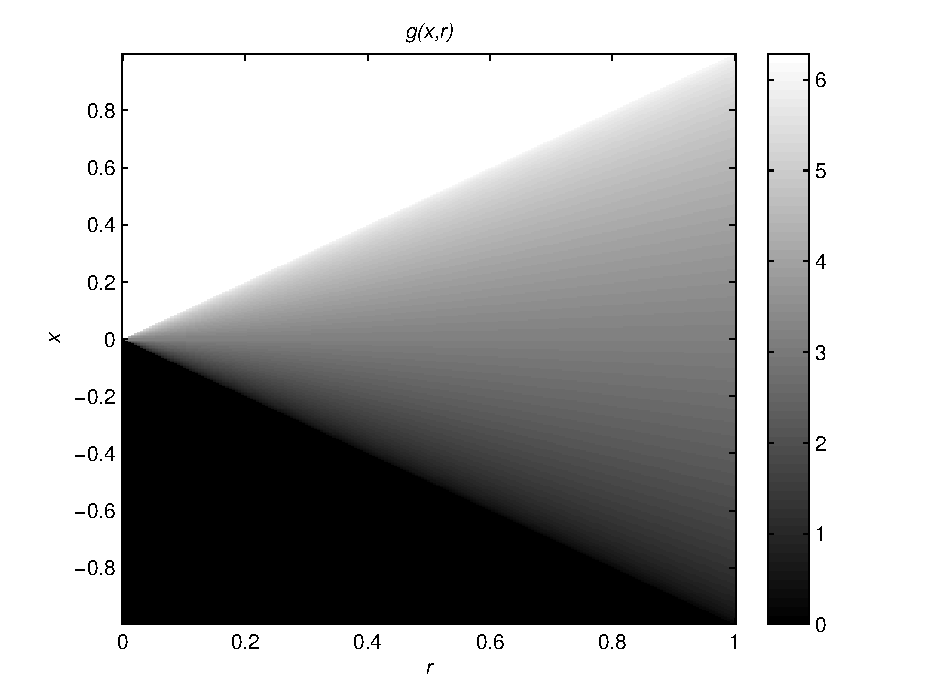
\includegraphics[width=.5\textwidth]{figures/g_function.pdf}
\end{center}
\caption{ The PSF forward integral operator kernel $g(x,r)$ represented as the arc measure of $v$ in $(-\pi,\pi)$ where $x \ge r\cos v$. }\label{fig:radialForwardKernel}
\end{figure}


\begin{figure}
  \begin{center}
    \begin{tikzpicture}[scale=.8,every node/.style={minimum size=1cm},on grid]
      \def\myxslant{0.1}
      \def\myyslant{-0.4}

	\begin{scope}[
		xshift=40,
		every node/.append style={
		xslant=\myxslant,yslant=\myyslant},xslant=\myxslant,yslant=\myyslant
	]
	\draw (0,0) rectangle (2.8,2.2);
%	\draw[fill=black] (1,0) rectangle (2.8,2.2);
	\end{scope}

	\begin{scope}[
		yshift=-20,
		every node/.append style={xslant=\myxslant,yslant=\myyslant},
		xslant=\myxslant,yslant=\myyslant
	]
	\draw[x=.314cm,y=.2cm,z=.2cm,thick,-latex,red] (0,0,0)
	  sin ++(0,1,1) cos ++(0,-1,1) sin ++(0,-1,1) cos ++(0,1,1)
	  sin ++(0,1,1) cos ++(0,-1,1) sin ++(0,-1,1) cos ++(0,1,1)
	  sin ++(0,1,1) cos ++(0,-1,1) sin ++(0,-1,1) cos ++(0,1,1);
	\draw[x=.314cm,y=.2cm,z=.2cm,thick,-latex,red] (-2,0,0)
	  sin ++(0,1,1) cos ++(0,-1,1) sin ++(0,-1,1) cos ++(0,1,1)
	  sin ++(0,1,1) cos ++(0,-1,1) sin ++(0,-1,1) cos ++(0,1,1)
	  sin ++(0,1,1) cos ++(0,-1,1) sin ++(0,-1,1) cos ++(0,1,1);
	\draw[x=.314cm,y=.2cm,z=.2cm,thick,-latex,red] (-4,0,0)
	  sin ++(0,1,1) cos ++(0,-1,1) sin ++(0,-1,1) cos ++(0,1,1)
	  sin ++(0,1,1) cos ++(0,-1,1) sin ++(0,-1,1) cos ++(0,1,1)
	  sin ++(0,1,1) cos ++(0,-1,1) sin ++(0,-1,1) cos ++(0,1,1);

	\pgfmathsetmacro{\cubex}{2}
	\pgfmathsetmacro{\cubey}{2.5}
	\pgfmathsetmacro{\cubez}{1}
	\draw[black,fill=gray,opacity=.75] (3.7,3,0) -- ++(-\cubex,0,0) -- ++(0,-\cubey,0) -- ++(\cubex,0,0) -- cycle;
	\draw[black,fill=gray,opacity=.75] (3.7,3,0) -- ++(0,0,-\cubez) -- ++(0,-\cubey,0) -- ++(0,0,\cubez) -- cycle;
	\draw[black,fill=gray,opacity=.75] (3.7,3,0) -- ++(-\cubex,0,0) -- ++(0,0,-\cubez) -- ++(\cubex,0,0) -- cycle;

	\draw[x=.314cm,y=.2cm,z=.2cm,thick,-latex,red] (4,0,0)
	  sin ++(0,1,1) cos ++(0,-1,1) sin ++(0,-1,1) cos ++(0,1,1)
	  sin ++(0,1,1) cos ++(0,-1,1) sin ++(0,-1,1) cos ++(0,1,1);
	\draw[x=.314cm,y=.2cm,z=.2cm,thick,-latex,red] (2,0,0)
	  sin ++(0,1,1) cos ++(0,-1,1) sin ++(0,-1,1) cos ++(0,1,1)
	  sin ++(0,1,1) cos ++(0,-1,1) sin ++(0,-1,1) cos ++(0,1,1);
	\end{scope}

	\begin{scope}[
		xshift=180,
		every node/.append style={xslant=\myxslant,yslant=\myyslant},
		xslant=\myxslant,yslant=\myyslant
	]
	    \draw (0,0) rectangle (2.8,2.2);
	    \tikzfading[name=fade left,left color = transparent!100,right color = transparent!0]
	    \draw[path fading=fade left,fading transform={rotate=-30},fill=black] (.9,0) rectangle (1,2.2);
	    \draw[fill=black] (1,0) rectangle (2.8,2.2);
	\end{scope}

	\begin{scope}[
		xshift=300,
		every node/.append style={xslant=\myxslant,yslant=\myyslant},
		xslant=\myxslant,yslant=\myyslant
		]
	    \draw (0,0) rectangle (2.8,2.2);
	    \tikzfading[name=fade left,left color = transparent!100,right color = transparent!0]
	    \draw[path fading=fade left,fading transform={rotate=-30},fill=black] (.9,0) rectangle (1,2.2);
	    \draw[fill=black] (1,0) rectangle (2.8,2.2);
	    \draw[step=1mm, black] (0,0) grid (2.8,2.2); %defining grids
	\end{scope}
	

    %    %putting arrows and labels:
	\node at (2,2.5) (label1) {Opaque Edge};
	\draw[-latex,thick] (2,-2) to node[below] {Image System Response} (7.5,-2);
	\node at (4.65,-3.4) (math1) {$\displaystyle{b(x)=\iint_{\Omega} k(s,t) f(x-s)\,dsdt}$};

	\node at (7,2.5) (label3) {Blurred Profile};

	\node at (12,2.5) (label2) {Recorded Data};
	\draw[-latex,thick] (9,-2) to node[below]{Measurement error} (13.2,-2);
	\node at (11,-3.4) (math1) {$+\eps_x \sim N(0, \sigma^2)$};

    \end{tikzpicture}
  \caption{ A schematic of the measurement model for an X-Ray image of an edge. An opaque block aligned with the imaging plane blocks light on the half plane to produce a blurred edge.}\label{fig:edgePicture}
\end{center}
\end{figure}

\begin{figure}
\begin{center}
  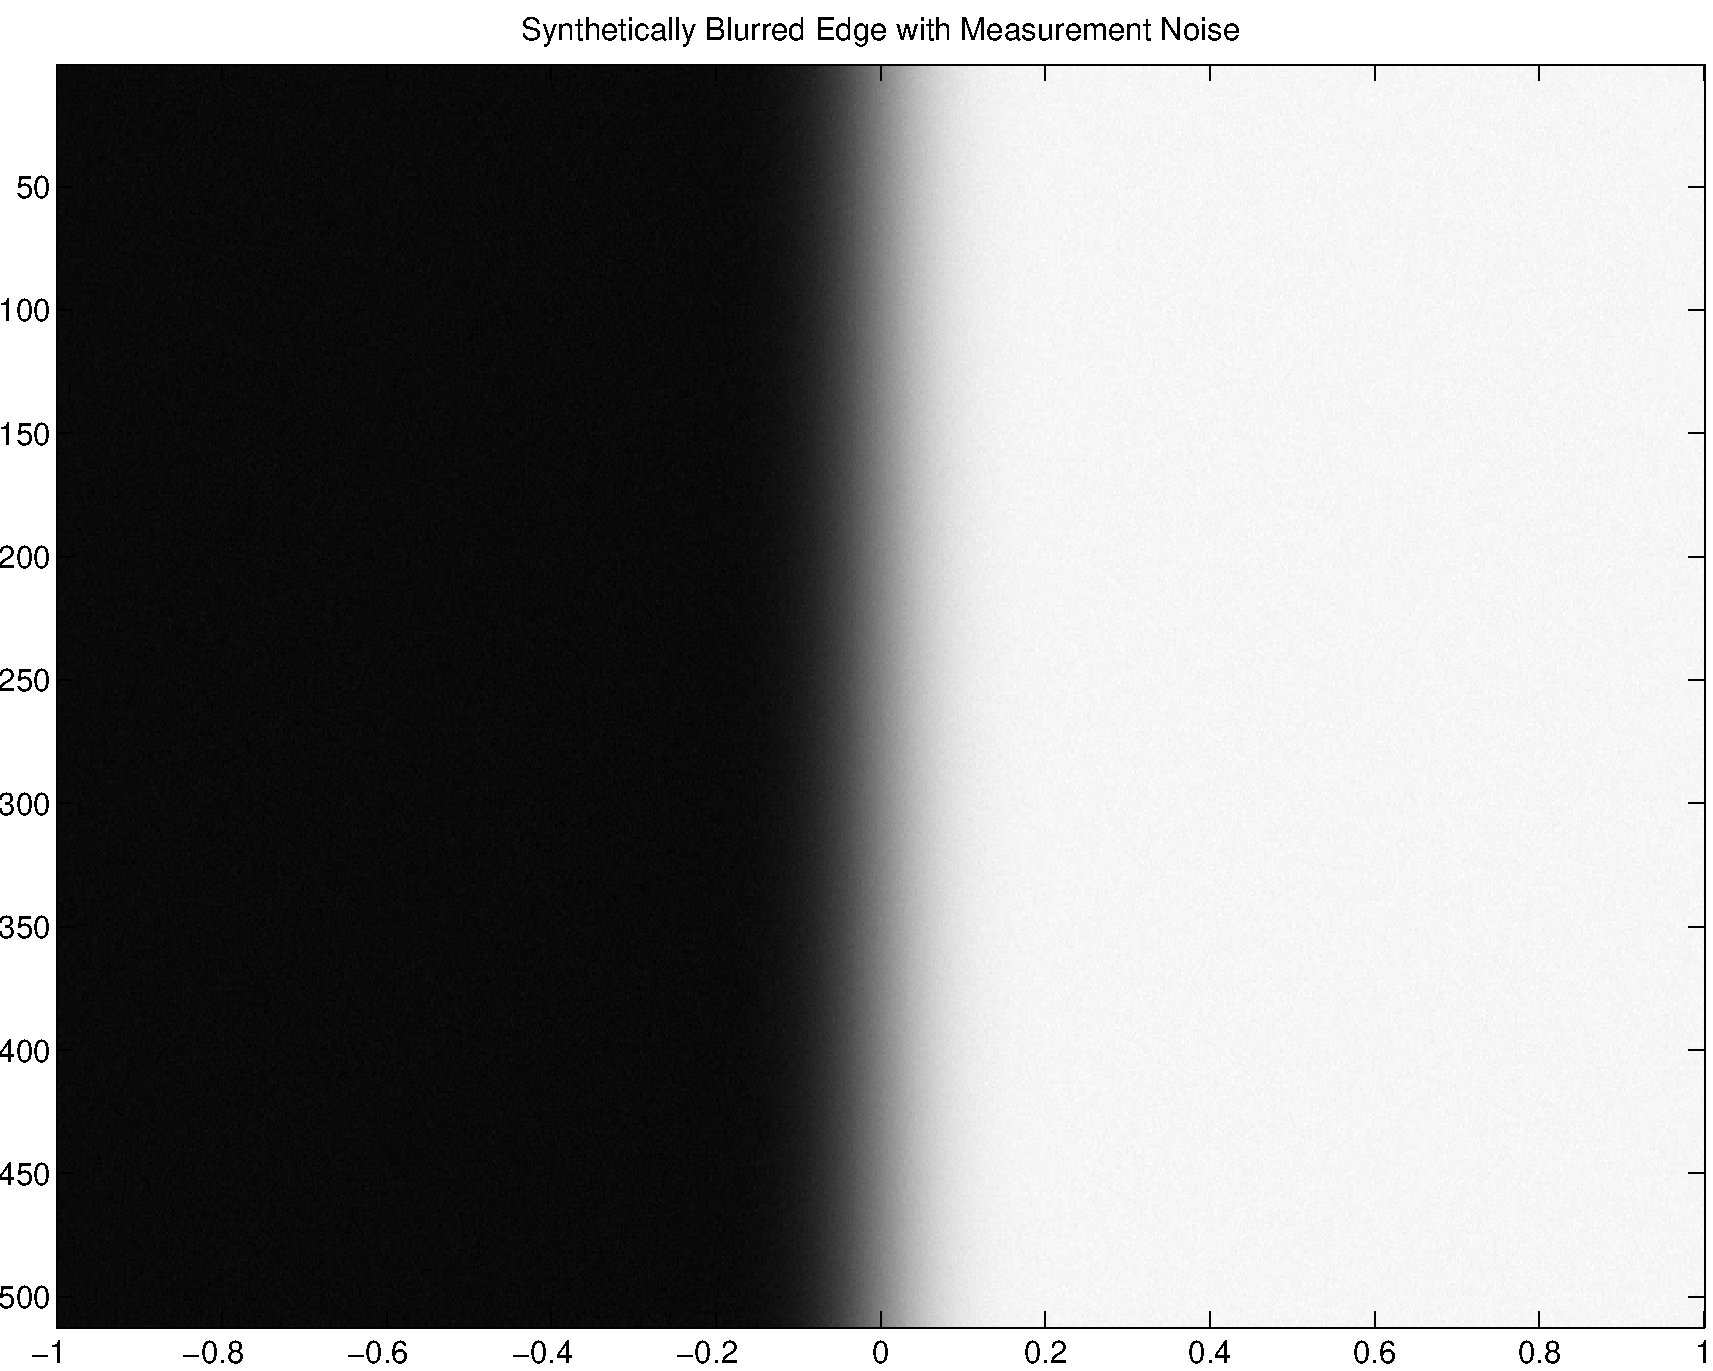
\includegraphics[width=.45\textwidth]{figures/blurredEdgeData.pdf}
  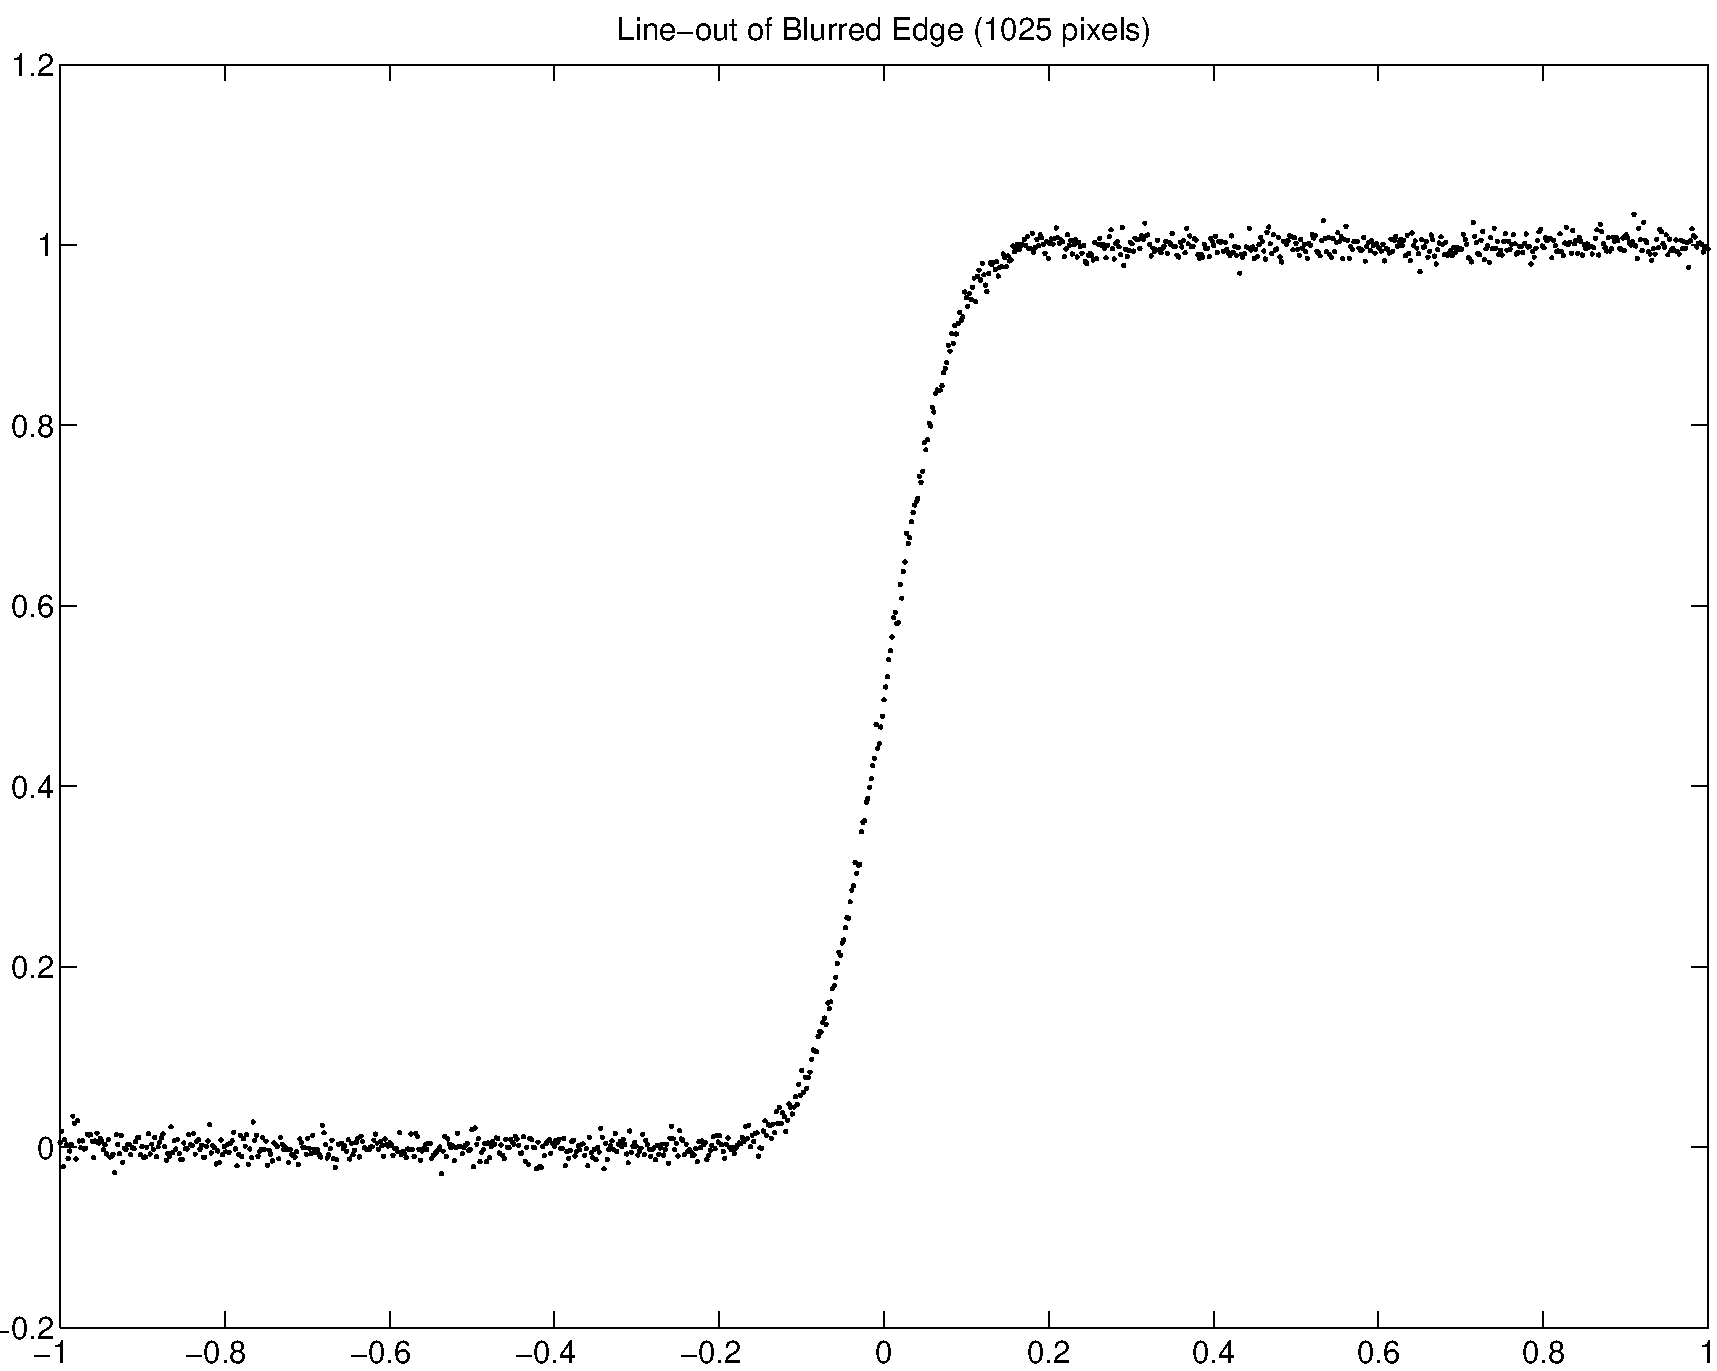
\includegraphics[width=.45\textwidth]{figures/psfLineoutData.pdf}
  \caption{A synthetically blurred edge with simulated measurement error and a line-out (horizontal cross-section) from the data.} \label{fig:edgeData}
\end{center}
\end{figure}

  
\section{Organization}
  In the next chapter, we will give a basic outline of Bayesian estimation techniques for the problem of PSF reconstruction.
  Primarily, we will develop the theoretical framework of how inference can be carried out on the radial profile of the PSF, when prior assumptions are placed on the PSF itself.
  Chapter 2 will be mainly theoretical, but the explicit forms for the discrete model of the forward operator and prior are motivated and derived there.
  Chapter 3 will give details on how to carry out the estimation on a computer.
  There, we will deal with how to discretely represent each of the necessary components in the estimation problem.
  We will also motivate and present the design of a detailed algorithm for carrying out the estimation outlined in Chapter 2.
  Finally, in Chapter 4, we present the results of an implementation on synthetically derived data and on measured data from a high-energy X-ray imaging system at the U.S.~Department of Energy's Nevada National Security Site.
  We will end with a discussion of conclusions and possible future work.


\end{chapter}
  % This line will include the file "chapter1.tex"  You must include a
                        % similar line for each chapter.  Each chapter should be in its own file
                        % and the file name should be descriptive (instead of just chapter1,
                        % chapter2 etc.).
\setlength{\parindent}{2ex}
%\newcommand{\mathscr}{\mathcal}
\begin{chapter}{Reconstruction on the Continuum}\label{chapter:theoretical}

The goal of this chapter is to develop the necessary mathematical tools to encapsulate prior notions of both smoothness and radial symmetry within the structure of a separable Hilbert space.
This is done within the framework of distributions from linear PDE theory. 

\begin{com}
  There is enough structure here to do what we want and maintain the structure of a Hilbert space. 
  This will make rigorous the discussion at the end of the last chapter for showing that the problem is ill-posed.
  It will also allow us to give rigorous formal definition for an infinite dimensional stochastic formulation of the problem.
  This will be the basis for estimation in the following chapter.
\end{com}

\section{Distribution spaces}
In this section we establish the preliminary definitions and main results from distribution theory.
There are several treatments of the subject in varying levels of generality, and this work draws primarily from \citep{richtmyer1978principles,hormander1983,rudin1991,griffel2002,strichartz2003guide}.

  \subsection{The space of test functions and distributions}

\begin{com}
The space of distributions provides  blah blah, a bunch of bullshit from PDEs and incidentally integral equations.
\end{com}

Let $\DD(\Omega)$ be the space of compactly supported smooth functions defined on an open set $\Omega \subseteq \R^k$.
Endow $\DD(\Omega)$ with the topology such that $(\phi_n)\subset \DD(\Omega)$ converges there exists a compact set $K$ such that 
\begin{equation}
  \bigcup_{n=1}^\infty \supp \phi_n \subseteq K \quad\text{and}\quad
  \sup_{m\ge n} \left|\del^\alpha (\phi_n-\phi_m)\right|\to 0, \label{eq:testFunctionContinuity}
\end{equation} 
for any multi-index such that $|\alpha|\le k$.
That is,  $\alpha$ is a $k$-tuple of non-negative integers $(\alpha_1\dots \alpha_k)$, such that $\sum \alpha_i \le k$ and $\del^\alpha = \prod \left(\frac{\del}{\del x_i}\right)^{\alpha_i}$.
In distribution theory, these are called \emph{test functions} on $\Omega$.
The space of continuous linear functionals, denoted $D^*(\Omega)$, are the \emph{distributions} on $\Omega$.
We adopt the notation $\langle f, \phi\rangle$ for the action of a linear functional $f$ on $\phi \in \DD(\Omega)$ and freely use the natural inclusion of functions $g \to \tilde g \in \DD^*(\Omega)$ by $\langle \tilde g, \phi \rangle = \int g\, \phi\,dx$ when the integration exists and omit the tilde notation distinguishing $g$ and $\tilde g$ as the representation should be clear from context. 

We state two general topological results regarding distributions. See \citep[Chapter 2]{hormander1983} for the proofs of each.
\begin{thm} \label{thm:completeness}
  Suppose $(f_n)$ is a sequence in $\DD^*(\Omega)$ such that $\lim\langle f_n,\phi\rangle$ exists for all $\phi \in \DD(\Omega)$, then there exists a unique $f\in \DD^*(\Omega)$ such that
  \begin{equation}
    \langle f, \phi\rangle = \lim_{n\to\infty} \langle f_n, \phi \rangle.
  \end{equation}
\end{thm}
The existence of such of the bilinear form $f$ can be readily established by using the completeness of the associated field, either $\R$ or $\C$, and the main difficulty of establishing the result is showing that the resulting linear functional is continuous on $\DD(\Omega)$.

The next result, sometimes referred to as localization, establishes a dense embedding of the $\DD(\Omega)$ into $\DD^*(\Omega)$.
\begin{thm} \label{thm:density}
  Given $f\in \DD^*(\Omega)$, there exists a sequence $(\phi_n) \subset \DD(\Omega)$ such that 
  \begin{equation}
    \langle f,\psi\rangle = \lim_{n\to\infty}\langle \phi_n,\psi\rangle.
  \end{equation}
\end{thm}

These results allow for operators defined on $\DD(\Omega)$ to be extended in a continuous way to $\DD^*(\Omega)$ so long as one can define an adjoint operation with respect to the bilinear form $\langle \cdot,\cdot \rangle$.
The classical example is extending the differential operator $\frac{\del}{\del x_i}:\DD^*(\Omega) \to \DD^*(\Omega)$. 
First, for test functions observe that integrating by parts and using the compactness of the support of $\psi$ yields
\begin{equation}
  \left\langle \frac{\del}{\del x_i} \phi,\psi \right\rangle = \int_{\Omega} \frac{\del}{\del x_i} \phi(x) \psi(x) dx = - \int_{\Omega}\phi(x) \frac{\del}{\del x_i} \psi(x)dx =- \left\langle \phi, \frac{\del}{\del x_i} \psi\right\rangle.
\end{equation}
This motivates defining $\frac{\del}{\del x_i} f \in \DD^*(\Omega)$ by
\begin{equation}
  \left\langle \frac{\del}{\del x_i} f, \phi \right\rangle 
    \eqdef  - \left\langle f, \frac{\del}{\del x_i} \psi\right\rangle
\end{equation}
from which we can extend the definition of $\del^\alpha$
\begin{equation}\label{eq:distributionalDerivative}
  \left\langle \del^\alpha f, \phi \right\rangle 
    \eqdef  (-1)^{|\alpha|} \left\langle f, \del^\alpha \psi\right\rangle.
\end{equation}
For a given sequence $(\phi_n)\subset \DD(\Omega)$ converges uniformly in all derivatives, the functional defined in \eqref{eq:distributionalDerivative} is continuous, hence is in $\DD^*(\Omega)$.
Since the operator $\del^\alpha:\DD^*(\Omega)\to\DD^*(\Omega)$ is expressed as an adjoint on test functions with respect to evaluation, its continuity follows directly from the weak-topology induced from $\DD(\Omega)$, i.e., suppose $f_n \to f$ in $\DD^*(\Omega)$, then
\begin{align}
  \lim_{n\to \infty}\langle \del^{\alpha}f_n, \phi\rangle 
  = \lim_{n\to\infty}(-1)^{|\alpha|} \langle f_n,\del^{\alpha}\phi\rangle
  = (-1)^{|\alpha|} \langle f,\del^{\alpha}\phi\rangle
  = \langle \del^{\alpha}f, \phi\rangle.
\end{align}

This approach serves as a template for how we will extend the radial change of variables in \Cref{chapter:introduction} to larger spaces of distributions.

\subsection{$L^2$ as a subspace of distributions}

\begin{com}
  We need metrics and norms and algebra to play nice together.
  The best space for that is a Hilbert space, and in particular a closed substace of $L^2$.
  Here we show how to view the space of $L^2$ functions as a subspace of $\DD^*$.
\end{com}
The development follows \citep{richtmyer1978principles}, for which we need only the notion the $L^2$ inner product, as opposed to Fourier based approaches which can be found in \citep{rudin1991,hormander1983}.
This development provides several details that are omitted in \citep{richtmyer1978principles}. 

We define the $L^2$ inner-product for test functions as the bilinear form $(\cdot,\cdot)_{L^2(\Omega)}:\DD(\Omega)\times\DD(\Omega) \to \C$ by 
\begin{equation} \label{eq:l2innerProduct}
  (\phi,\psi)_{L^2(\Omega)} \eqdef \int_{\Omega} \phi(x)\bar{\psi(x)}\,dx,
\end{equation}
with the induced norm 
\begin{equation} \label{eq:l2norm}
  \|\phi\|^2_{L^2(\Omega)} \eqdef (\phi,\phi)_{L^2(\Omega)}.
\end{equation}
The linearity of \eqref{eq:l2innerProduct} is inherited by the linearity of integration and positivity follows from the positivity of $\phi(x)\bar{\phi(x)} = |\phi(x)|^2$. 
For definiteness, note that if $\phi = 0$ then $\|\phi\|_{L^2(\Omega)} = 0$, and only if $\phi = 0$, otherwise, continuity of $\phi$ implies a neighborhood where $|\phi(x)| > 0$ which gives $\|\phi\|_{L^2(\Omega)} > 0$.
Since \eqref{eq:l2innerProduct} defines an inner-product, the triangle inequality of the norm follows from the Cauchy-Schwarz-Bunyakovsky inequality.

A sequence $(\phi_n)\subset \DD(\Omega)$ is Cauchy with respect to $L^2(\Omega)$ if
\begin{equation} 
  \sup_{k\ge n} \|\phi_n - \phi_k\|_{L^2(\Omega)} \to 0.
\end{equation}
Observe that $(\phi,\psi)_{L^2(\Omega)} = \langle \phi,\bar{\psi}\rangle$ when $\phi$ is viewed as an element of $\DD^*(\Omega)$.
Hence, if $(\phi_n)$ is Cauchy with respect to $L^2(\Omega)$, then the sequence $\big(\langle \phi_n,\psi\rangle\big)$ is a Cauchy sequence of complex numbers, i.e., using Cauchy-Schwarz-Bunyakovsky
\begin{equation}
  |\langle \phi_n, \psi \rangle - \langle \phi_k,\psi\rangle| 
    = |(\phi_n - \phi_k,\bar{\psi})_{L^2(\Omega)}|  
    \le \|\phi_n - \phi_k\|_{L^2(\Omega)}\|\psi\|_{L^2(\Omega)}. \label{eq:cauchySchwarz}
\end{equation}
Hence, $\lim\langle \phi_n,\psi\rangle$ exists for all $\psi \in \DD(\Omega)$ (by completeness of $\C$), and \Cref{thm:completeness} provides uniquely an $f \in \DD^*(\Omega)$ such that
\begin{equation}
  \lim_{n\to\infty} \langle \phi_n, \psi\rangle = \langle f,\psi\rangle.
\end{equation}
All such $f$ are elements of the space $L^2(\Omega)$.

Sequences $(\phi_n)$ and $(\psi_n)$ are \emph{equivalent} $L^2(\Omega)$ Cauchy sequences if
\begin{equation}\label{eq:cauchyEquivalence}
  \|\phi_n - \phi_n'\|_{L^2(\Omega)} \to 0.
\end{equation}
These distributions are well defined in the following sense: 
\begin{prop} \label{prop:cauchyCorrespondence}
  Sequences $(\phi_n)$ and $(\phi_n')$ determine the same distribution if and only if they are equivalent.
\end{prop}
\begin{proof}
  Suppose $(\phi_n)$ and $(\phi_n')$ are equivalent Cauchy sequences for $f$ and $f'$ respectively.
  Arguing similarly to \eqref{eq:cauchySchwarz},
  \begin{align} 
    |\langle f, \psi\rangle - \langle g, \psi\rangle| = \left|\lim_{n\to \infty}\langle \phi_n - \phi_n', \psi\rangle\right| \le \lim_{n\to\infty}\|\phi_n - \phi_n'\|_{L^2(\Omega)}\|\psi\|_{L^2(\Omega)} =  0
  \end{align} 
  for all $\psi \in \DD^(\Omega)$, hence $f = f'$.

  Conversely, suppose $(\phi_n)$ and $(\phi_n')$ are Cauchy sequences that determine the same distribution $f$, hence
  \begin{equation}
    \lim_{n\to\infty} \langle \phi_n,\psi\rangle = \lim_{n\to\infty} \langle \phi_n',\psi\rangle = \langle f,\psi\rangle
  \end{equation}
  for all $\psi \in \DD^*(\Omega)$.
  The sequence given by $\xi_n = \phi_n - \phi_n'$ is also Cauchy by the triangle inequality, and 
  \begin{equation}
    \lim_{n\to\infty}\langle \xi_n,\bar{\psi}\rangle^2 = \lim_{n\to\infty} (\xi_n,\psi)_{L^2(\Omega)}^2 = 0.
  \end{equation}
  Let $\eps >0$ be given and $n_0$ sufficiently large such that 
  \begin{equation}
    \sup_{k\ge n_0} \|\xi_{n_0} - \xi_k\|_{L^2(\Omega)}^2 < \eps.
  \end{equation}
  Using Cauchy-Schwarz-Bunyakovsky,
  \begin{align}
    \|\xi_n\|_{L^2(\Omega)}^2 
      &= |(\xi_n,\xi_n)_{L^2(\Omega)}| \nonumber\\
      &= |(\xi_n,\xi_n - \xi_{n_0})_{L^2(\Omega)}| \nonumber\\
      &\le \|\xi_n\|_{L^2(\Omega)}\|\xi_n-\xi_{n_0}\|_{L^2(\Omega)}
  \end{align}
  we have that for all $\|\xi_n\|_{L^2(\Omega)} \not= 0$
  \begin{equation}
    \|\xi_n\|_{L^2(\Omega)} \le \|\xi_n - \xi_{n_0}\|_{L^2(\Omega)} < \eps
  \end{equation}
  for all $n \ge n_0$, hence $\|\xi_n\|_{L^2(\Omega)} \to 0$ which implies $\phi_n$ and $\phi_n'$ are equivalent Cauchy sequences.
\end{proof}

It can be readily shown that \eqref{eq:cauchyEquivalence} defines an equivalence relation on Cauchy sequences for which vector addition and scalar multiplication are well-defined, hence, the equivalence classes of Cauchy sequences form linear subspace of $\DD^*(\Omega)$.

We can now extend the inner product to elements in $L^2(\Omega)$ in the following way,
\begin{equation} \label{eq:l2innerProductFull}
  (f,g)_{L^2(\Omega)} \eqdef \lim_{n\to\infty} (\phi_n,\psi_n)_{L^2(\Omega)}
\end{equation}
where $(\phi_n)$ and $(\psi_n)$ are Cauchy sequences corresponding to $f$ and $g$ respectively.
\begin{prop}
  The limit in \eqref{eq:l2innerProductFull} exists and is well-defined for equivalent Cauchy sequences. 
  Moreover, $\lim_{n\to\infty} \langle f,\bar{\psi_n}\rangle _{L^2(\Omega)} = (f,g)_{L^2(\Omega)}$.
\end{prop}
\begin{proof}
  Since $(\phi_n)$ and $(\psi_n)$ are Cauchy, the inequality $|\|\phi_n\|_{L^2(\Omega)} - \|\phi_k\|_{L^2(\Omega)}| \le \|\phi_n - \phi_k\|_{L^2(\Omega)}$ implies that $\|\phi_n\|_{L^2(\Omega)}$ and $\|\psi_n\|$ are both Cauchy sequences of positive numbers, and thus have finite limits.

Now observe,
\begin{align}
  |(\phi_n,\psi_n)_{L^2(\Omega)} - (\phi_k,\psi_k)_{L^2(\Omega)}| 
    &= (\phi_n,\psi_n-\psi_k)_{L^2(\Omega)} -(\phi_n-\phi_k,\psi_k)_{L^2(\Omega)}| \nonumber\\
    &\le \|\phi_n\|_{L^2(\Omega)}\|\psi_n-\psi_k\|_{L^2(\Omega)} + \|\phi_n - \phi_k\|_{L^2(\Omega)}\|\psi_k\|_{L^2(\Omega)} \nonumber\\
    &\le \|\phi_n\|_{L^2(\Omega)}\|\psi_n-\psi_k\|_{L^2(\Omega)} \nonumber\\
    &\quad\quad+ \|\phi_n - \phi_k\|_{L^2(\Omega)}\big(\|\psi_k - \psi_n\|_{L^2(\Omega)} + \|\psi_n\|_{L^2(\Omega)}\big)
\end{align}
and taking $\sup_{k\ge n}$ then limiting in $n$ on the right hand side of the inequality results in 0 since $(\|\phi_n\|)$ and $(\|\psi_n\|$ have finite limits.
Thus, $(\phi_n,\psi_n)$ is a Cauchy sequence in $\C$, and hence, has a finite limit.

Let $\eps > 0$ be given. 
For all $n$, choose $m$ sufficiently large so that
\begin{align}
  |\langle f,\bar{\psi_n}\rangle - (f,g)_{L^2(\Omega)}| 
    &\le |\langle f - \phi_m,\bar{\psi_n}\rangle| + |\langle \phi_m - \phi_n, \bar{\psi_n}\rangle| + |\langle \phi_n,\bar{\psi_n}\rangle - (f,g)_{L^2(\Omega)}| \nonumber\\
    &\le |\langle f - \phi_m,\bar{\psi_n}\rangle| + \| \phi_m - \phi_n\| \|\psi_n\| + |\langle \phi_n,\bar{\psi_n}\rangle - (f,g)_{L^2(\Omega)}| \nonumber\\
    &< \eps +|\langle \phi_n,\bar{\psi_n}\rangle - (f,g)_{L^2(\Omega)}|.
\end{align}
Taking limits on both sides gives 
\begin{equation} \label{eq:iteratedInnerProduct}
  \lim_{n\to\infty} \langle f,\bar{\psi_n}\rangle = (f,g)_{L^2(\Omega)}, 
\end{equation}
since $\eps>0$ is arbitrary.

Finally, to show that the inner product is well-defined, suppose $(\phi_n')$ and $(\psi_n')$ are equivalent Cauchy sequences to $(\phi_n)$ and $(\psi_n)$ respectively.
\begin{align}
%  |(f,g) - (f',g')| \lim_{n\to\infty}
%  |(\phi_n,\psi_n)_{L^2(\Omega)} - (\phi_n',\psi_n')_{L^2(\Omega)}|
%  &=|(\phi_n,\psi_n - \psi_n')_{L^2(\Omega)} - (\phi_n'-\phi_n,\psi_n')_{L^2(\Omega)}| \nonumber \\
%  &=|\langle\bar{\psi_n - \psi_n'},\phi_n\rangle - \langle\phi_n'-\phi_n,\bar{\psi_n'}\rangle| \label{eq:innerProductWellDefined}
%  = |(\phi_n - \phi_n',\phi_n - \phi_n') + (\psi_n - \psi_n',\psi_n - \psi_n') - (\phi_n',\psi_n')|
  |\lim_{n\to\infty}(\phi_n,\psi_n)_{L^2(\Omega)} - (\phi_n',\psi_n')_{L^2(\Omega)}| 
  &= |\lim_{n\to\infty}\langle f,\bar{\psi_n}\rangle - \lim_{n\to\infty}\langle f',\bar{\psi_n}'\rangle| &\text{by \eqref{eq:iteratedInnerProduct}}\nonumber\\
  &= |\lim_{n\to\infty}\langle f,\bar{\psi_n} - \bar{\psi_n}'\rangle| &\text{by \Cref{prop:cauchyCorrespondence}}\nonumber \\
  &= 0 \nonumber.
\end{align}
Thus, the inner product is well-defined for equivalent Cauchy sequences.
\end{proof}

Showing that \eqref{eq:l2innerProductFull} is an inner product on $L^2(\Omega)$ is straight-forward, and the resulting inner product space is a Hilbert space, as stated in the following theorem.
\begin{thm}
The space $L^2(\Omega)$ is complete complete with respect to the inner product defined in \eqref{eq:l2innerProductFull}, hence, is a Hilbert space.
\end{thm}
%\begin{proof}
%  Let $(f_n)\subseteq $ be a Cauchy sequence with respect to \eqref{eq:l2innerProductFull}. 
%\end{proof}
See \citep{richtmyer1978principles} for the proof, which follows a standard diagonalization argument. %similar to the Arzela-Ascoli theorem.
We remark that there is a correspondence with the standard notion of $L^2(\Omega)$ with respect to Lebesgue measure and this development.
The basis of correspondence comes from the result that simple function can be arbitrarily approximated with a sequence of test functions in the standard $L^2(\Omega)$ sense with Lebesgue measure. 
See \citep{hormander1983} for a rigorous development of this correspondence.
%\begin{com}
%  Use the hard work in \Cref{thm:density} maybe.
%\end{com}
\subsection{The Sobolev spaces $\HH^n(\Omega)$ and $\HH_0^n(\Omega)$}
Sobolev spaces provide a framework for imposing regularity on distributions in terms of their derivatives.
In this subsection, we briefly overview the definition of these spaces, and state a version of the Sobolev embedding theorem sufficient for characterizing PSFs of interest in this work.

\section{Radial symmetry}
Symmetry is established by casting it in terms of a many-to-one smooth map $T$ that is constant on circles of a fixed radius.  
If $f$ is a function on $\R^2$ and there exists a function $\rho$ so that $f(x,y) = \rho(\sqrt{x^2 + y^2})$, then observe that $f$ has the common notion of radial symmetry with a radial profile $\rho$.
This notion is easily adapted to distributions by developing the corresponding linear pullback operator to $T^\sharp$ that maps $\rho$ to $f$ by precomposition by $T(x,y)$ on sequences of test functions converging to $\rho$.

\subsection{The pull-back operator}
In this subsection, we will explicitly construct the pullback operator $T^\sharp$ for a slightly more general smooth map $T(x,y)$. 
It will turn out that our choice of $T$ will induce a pullback operator that is injective.
This is the content of the following theorem.

This is the content of the following theorem.
\begin{thm} \label{thm:pullback}
  Let $\Omega_1 := (0,\infty) \subset \R$ and $\Omega_2 := \R^2 \setminus \{x = 0\text{ or }y=0\}$.
  For $h:\Omega_1\to\Omega_1$ such that $h(t) = t^a$ for $0<a<1$, let $T:\Omega_2 \to \Omega_1$ by $T(x,y) = h(x^2 + y^2)$, then there exists a unique, injective, continuous, linear operator $T^\sharp:\DD^*(\Omega_1) \to \DD^*(\Omega_2)$ so that $\langle T^\sharp \rho ,\phi\rangle = \langle \rho \circ T,\phi\rangle$ for all $\phi \in \DD(\Omega_2)$ and $\rho \in \DD(\Omega_1)$.
\end{thm}

To prove this result, we first establish the following lemmas.

\begin{lem} \label{lem:existence}
  There exists a map $T_{\sharp}:\DD(\Omega_2) \to \DD(\Omega_1)$ so that for any $\rho \in \DD(\Omega_1)$
  \begin{equation}
    \langle \rho \circ T, \phi \rangle_{\Omega_2} = \langle \rho, T_\sharp \phi\rangle_{\Omega_1}.
  \end{equation}
\end{lem}
\begin{proof}
  Let $Q_{ij} = \{ (x,y): (-1)^i x>0, (-1)^jy>0\}$ for $i,j \in \{0,1\}$ so that $\bigcup Q_{ij} = \Omega_2$.
  Define $T_{ij}:Q_{ij} \to R\subset \R^2$ by 
  \begin{equation}
    T_{ij}(x,y) = \Big(T(x,y), (-1)^jy\Big). 
  \end{equation}
  Observe that each $T_{ij}$ is a diffeomorphism onto $R = \left\{(r,t): 0 < t < \sqrt{h^{-1}(r)}\right\} = \left\{(r,t): 0 < t < r^{\frac{1}{2a}}\right\}$ with inverse 
  \begin{align}
    T_{ij}^{-1}(r,t) 
      &= \Big((-1)^i\sqrt{h^{-1}(r) - t^2}, (-1)^jt\Big),\nonumber\\
      &= \Big((-1)^i\sqrt{r^{\frac 1a} - t^2}, (-1)^jt\Big),\\
    \intertext{ and }
    \left|dT_{ij}^{-1}(r,t)\right| 
      &= \frac12 \frac{\del}{\del r}[h^{-1}(r)]\left(h^{-1}(r) - t^2\right)^{-1/2}\nonumber \\
      &= \frac{1}{2a} r^{\frac 1a-1}\left(r^{\frac 1a} - t^2\right)^{-1/2}, \label{eq:determinant}
  \end{align}
  which is positive and smooth for all $(r,t)\in \Omega_2$.
  Furthermore, note that 
  \begin{equation}
    T \circ T_{ij}^{-1}(r,t) = r. \label{eq:partialInverseT}
  \end{equation}
  Now, given $\rho \in \DD(\Omega_1)$, a change of variables results in
  \begin{align}
    \langle \rho \circ T, \phi\rangle_{\Omega_2} 
%    &= \iint_{\Omega_2} \rho\circ T(x,y) \phi(x,y)dxdy \\
    &= \sum_{ij}\iint_{Q_{ij}} \rho\circ T(x,y)\cdot \phi(x,y)dxdy \nonumber \\
    &= \sum_{ij}\iint_{R} \rho(r)\cdot  \phi \circ T_{ij}^{-1}(r,t)\left|dT_{ij}\right|drdt \nonumber \\
    &= \int_0^\infty \rho(r) \left(\int_0^{\sqrt{h^{-1}(r)}} \sum_{ij}\phi \circ T_{ij}^{-1}(r,t)\left|dT_{ij}\right|dt \right)dr \label{eq:phiEquation}.
%    &=: \int_{\Omega_1} \rho(r) \Phi_{\phi,T_{ij}}(r) dr. 
%    &= \langle \rho, \Phi_{\phi,T_{ij}} \rangle_{\Omega_1},
  \end{align}
  Let 
  \begin{align}
    [T_\sharp\phi](r) 
      &= \int_0^{\sqrt{h^{-1}(r)}} \sum_{ij}\phi \circ T_{ij}^{-1}(r,t)\left|dT_{ij}\right|dt \\
      &= \frac{r^{\frac 1a -1} }{2a}\sum_{ij}\int_0^{r^{\frac{1}{2a}}} \phi \left((-1)^i\sqrt{r^{\frac 1a} - t^2}, (-1)^jt\right) \left( r^{\frac 1a} - t^2 \right)^{-1/2} dt, \label{eq:psiPhiDef}
  \end{align}
  and we must show that $T_\sharp\phi \in \DD(\Omega_1)$.
  Note that $\supp \left(\phi \circ T_{ij}^{-1} \right) = T_{ij}( \supp \phi )$ is compact in $R$ as the continuous image a compact set, and since $T_{ij}$ is a diffeomorphism, $\phi \circ T_{ij}^{-1} \in \DD(\Omega_2)$. 
%  Moreover, integrating marginally over $t$ and summing over ${i,j}$ are smooth operations, so $\Phi_{\phi,T_{ij}}$ is smooth. 
%  The support of $\Phi_{\phi,T_{ij}}$ is the projection of the support of $\phi\circ T_{ij}^{-1}$, hence is compact.
%  Marginially integrating $\phi\circ T_{ij}^{-1}$ results in a test function, thus $\Phi_{\phi,T_{ij}} \in \DD(\Omega_1)$. 
  Since $\phi\circ T_{ij}^{-1}(r,t)$ is smooth, a standard result from analysis \cite[pg. 433]{strichartz2000} implies that $\int \phi \circ T_{ij}^{-1}(r,t)\,dt$ is a smooth function in $r$.  
  The support of this function is the projection of the support of $\phi\circ T_{ij}$ onto the second coordinate, and hence, is compact.
  Summing over $i,j$ results results in a compactly supported smooth function.

\end{proof}

  Using \Cref{lem:existence}, define
  \begin{defn}
    Let $T^\sharp:\DD^*(\Omega_1) \to \DD^*(\Omega_2)$ by
  \begin{equation}
    \langle T^\sharp \rho, \phi \rangle_{\Omega_2} := \langle \rho, T_\sharp\phi\rangle_{\Omega_1}.
  \end{equation}
  \end{defn}
  To see that $T^\sharp \rho \in \DD^*(\Omega_2)$ (i.e. acts continuously on $\DD(\Omega_2)$ as a linear functioal), let $\{\phi_n\} \to 0$ in $\DD(\Omega_2)$, so in particular ($\alpha = 0$ in \eqref{eq:testFunctionContinuity}), $\sup|\phi_n| \to 0$. 
  Then, by \eqref{eq:psiPhiDef}, $\sup |T_\sharp\phi_n| \to 0$, and thus $\langle \rho, T_\sharp\phi_n\rangle \to 0$ by the continuity of $\rho$. 
%  Moreover, if we take $\rho = Id_{\DD(\Omega_1)}$ the iden, then $\langle Id_{}$
%  $T_\sharp:\DD(\Omega_2) \to \DD(\Omega_1)$.

  The linearity and continuity of $T^\sharp$ follow directly from this definition.
  That is 
  \begin{align}
    \langle T^\sharp \rho_1 + \alpha T^\sharp \rho_2,\phi\rangle_{\Omega_2} 
    &= \langle T^\sharp\rho_1,\phi\rangle_{\Omega_2} + \alpha\langle T^\sharp\rho_2 ,\phi \rangle_{\Omega_2} \nonumber\\ 
    &= \langle \rho_1,T_\sharp\phi\rangle_{\Omega_1} + \alpha\langle \rho_2 ,T_\sharp\phi \rangle_{\Omega_1} \nonumber\\
    &= \langle T^\sharp(\rho_1+\alpha \rho_2),\phi\rangle_{\Omega_2} \label{eq:linearity} 
  \end{align} 
  and if $\langle \rho_n, \psi\rangle \to 0$ for all $\psi \in \DD(\Omega_1)$, then 
  \begin{equation}
    \langle T^\sharp \rho_n,\phi\rangle_{\Omega_2} = \langle \rho_n,T_\sharp\phi\rangle_{\Omega_1} \to 0.
  \end{equation}

%As a corollary to this result, we can establish the existence in the statement of \Cref{thm:pullback}. That is, define $T^\sharp:\DD^*(\Omega_1) \to \DD^*(\Omega_2)$ by 
Loosely speaking, the pullback by $T$ represents a change of variables from $(x,y)$ to $(r,v)$ by expanding the domain of $T$ to an invertible $T_{ij}(x,y)$ with the choice of $T_{ij}$ somewhat arbitrary.  
For example, another valid choice of $T_{ij}$, which is similar to a polar-coordinates transformation, would be $(T(x,y), \mathrm{Arg}(x,y))$.
When uniqueness of $T^\sharp$ is shown, it will allow us to freely choose any other change of variables such that $T \circ T_{ij}(r,v) = r$, and the analysis on $T$ will still be valid.
Our choice was such that the analysis is straight-forward, although we will make use of the polar-coordinate variable transformation later to define the forward operator on linear representations.
The existence and continuity of a pullback operator can be carried out much more generally for any smooth $T$ and is outlined in \cite{hormander1983}.
However, in this case, because of the specific form of $T$ under consideration, the induced pullback $T^\sharp$ is injective. 
This will be a consequence of the next lemma.
\begin{lem} \label{lem:innerProduct}
  For all $\rho\in\DD^*(\Omega_1)$ and $\psi \in \DD(\Omega_1)$, then 
  then
  \begin{equation}
    \langle T^\sharp \rho , \psi \circ T \rangle_{\Omega_2} = \pi \langle \rho,\psi \cdot {h^{-1}}'\rangle_{\Omega_1}.
  \end{equation}
  where ${h^{-1}}'$ is the derivative of the inverse of $h$ in \Cref{thm:pullback}. 
\end{lem}
\begin{proof}
  First, note that both $\psi \circ T$ and ${h^{-1}}'\cdot \psi$ are elements of $\DD(\Omega_1)$.  
  From \eqref{eq:determinant}, observe
  \begin{align}
    \int_0^{\sqrt{h^{-1}(r)}} \left|dT_{ij}\right(r,t)| dt 
    &= \frac{{h^{-1}}'(r)}2 \int_0^{\sqrt{h^{-1}(r)}}\left(h^{-1}(r) - t^2\right)^{-1/2}\nonumber\\
    &= \frac\pi4 {h^{-1}}'(r).
  \end{align}
  Invoking \Cref{thm:testFunDensity}, let $\{\rho_n\}$ be a sequence in $\DD(\Omega_1)$ converging to $\rho$ in $\DD^*(\Omega_1)$, then substituting $\rho_n$ for $\rho$ and $\psi \circ T$ for $\phi$ in \eqref{eq:phiEquation}, we have
  \begin{align}
    \langle T^\sharp \rho_n, \psi \circ T \rangle_{\Omega_2}  &= 4\int_0^\infty \rho_n(r) \psi(r)  \left(\int_0^{\sqrt{h^{-1}(r)}} \left|dT_{ij}\right| dt\right) dr \nonumber \\
      &= \pi \int_0^\infty \rho_n(r) \psi(r)\,{h^{-1}}'(r) dr \nonumber\\
      &= \pi \left\langle\rho_n, \psi  \cdot {h^{-1}}' \right\rangle_{\Omega_1}. \label{eq:pullbackInnerProd}
  \end{align}
  By continuity of $T^\sharp$, the desired equality is established.
\end{proof}

We can now proceed to prove \Cref{thm:pullback}.
\begin{proof}
  It remains to show that 

  Uniqueness is a consequence of \Cref{thm:testFunDensity}. That is, suppose $T^\dagger:\DD^*(\Omega_1) \to \DD^*(\Omega_2)$ is a continuous linear functional such that $\langle T^\dagger \rho,\phi \rangle = \langle \rho \circ T, \phi\rangle$ for all $\phi \in \DD(\Omega_2)$ whenever $\rho \in \DD(\Omega_1)$. Then, for any $\rho \in \DD^*(\Omega_1)$, let $\{\rho_n\}\subset \DD(\Omega_1)$ converge to $\rho$ (in the $\DD^*(\Omega_1)$ sense), so 
  \begin{equation}
    \left\langle (T^\sharp - T^\dagger)\rho,\phi\right\rangle_{\Omega_2} = \lim \langle T^\sharp\rho_n,\phi\rangle_{\Omega_2} - \lim \langle T^\dagger\rho_n,\phi\rangle_{\Omega_2} = 0.
  \end{equation}
  Hence $T^\sharp = T^\dagger$.
  
  It remains to show that $T^\sharp$ is injective. Suppose $\rho \in \DD^*(\Omega_1)$ is such that $T^\sharp \rho = 0$.
  %and let $\{\rho_n\}\subset \DD(\Omega_1)$ converge to $\rho$ in $\DD^*(\Omega)$. For any $\psi \in \DD(\Omega_1)$,
  By the inverse function theorem,
  ${h^{-1}}'(r) = \frac 1{h'(r)} > 0$ since $h$ is increasing.
  So, $h' \cdot {h^{-1}}' (r) = 1$.
  %Let $\tilde h(r) = \frac 1{ {h^{-1}}'(r) }$, so $\tilde h \cdot {h^{-1}}' \equiv 1$.
  By \Cref{lem:innerProduct}, for an aribitrary $\psi\in \DD(\Omega_1)$,
  \begin{equation}
    0 = \Big\langle T^\sharp \rho, (h' \cdot \psi) \circ T)\Big\rangle_{\Omega_2} = \Big\langle \rho, \psi\Big\rangle_{\Omega_1},
  \end{equation}
  thus $\rho$ is the zero distribution.  Hence, $T^\sharp$ has trivial kernel and as a linear map is injective.
  We have established all of the properties in \Cref{thm:pullback}.
\end{proof}

\subsection{Borel's theorem and a motivating example}
\subsection{Radial symmetry for $L^2(\Omega_2)$ and $\HH_0^n(\Omega_2)$}

\section{The PSF inverse problem}
\subsection{The edge-blur operator for radially symmetric PSFs}
\subsection{Variational formulation of PSF estimation}
\subsection{Infinite dimensional Bayesian formulation for PSF estimation}

\end{chapter}

\setlength{\parindent}{2ex}
\newcommand{\Ab}{{\bf A}}
\newcommand{\N}{\mathcal{N}}
\begin{chapter}{Markov Chains and Modified Gibbs Sampling}\label{chapter:mcmctheory}
\begin{com} 
  Talk about what the novel contributions are.
  Start with the big idea, NOT 'in this chapter we are going to...'
  Aaron: 1. generating a statistical algorithm for PSF estimation, 2. prove invariance of partial collapse.
  So split the chapter.
  what is `the inverse problem' ?
\end{com}

\begin{com}
Modeling random things means dealing with .
  As is the case in Bayesian methods, incorporating observed data often leads to intractable densities.
  The Markov chain and relevant ergodic theorem are introduced, then we present the Gibbs sampler.
\end{com}

Observation informed estimation within a stochastic model can be analytically intractable, especially when the model deviates from standard models for independent or systematically data.
This is especially the case in many Bayesian methods, where inference is typically drawn from a posterior distribution, usually known only up to a constant of normalization.
\emph{Monte Carlo} methods use psuedo-random simulation methods to construct a simulated sample in order to characterize and estimate statistics about the underlying intractable probability density.
This chapter is devoted to introducing Monte Carlo methods that take advantage of a stochastic structure known as a Markov Chain in order to perform inference.
In particular, we investigate modifications to the widely used Gibbs sampler, and present modifications that improve its convergence.
The main tool for inference is the ergodic theorem for Markov Chains, which is stated along with its requisite hypotheses in \Cref{sec:mcmcTheory}.
This development will establish an important necessary condition, the invariance of the Markov Chain which is crucial to appropriately applying ergodic based inference on the Markov Chain.

We derive the standard Gibbs sampling algorithm, outlined by \citep{geman1984stochastic}, and present a modification using a technique called \emph{partial collapse}, which can motivated by several recent theoretical and practical analyses \citep{van2008partially,agapiou2014analysis,fox2015fast}.
This chapter gives a full development from first principles, and proves the assertions of invariance stated in \citep{van2008partially}, but not explicitly shown there.
We will also briefly review standard convergence diagnostics for comparing Markov Chain based sampling algorithms, which will establish statistical benchmarks to show that the adapted algorithm is indeed an enhancement of standard Gibbs sampling when applied to PSF estimation.  
\Cref{chapter:computational} will apply this general framework to the Bayesian PSF estimation problem.

\section{Markov Chain Monte Carlo Simulation} \label{sec:mcmcTheory}
In this section we give an overview of Markov Chain Monte Carlo (MCMC) methods for analyzing a probability distribution known up to a scaling constant.
Statistical analysis is based on the ergodic theorem for Markov chains, which can be thought of as the analogous notion to the central limit theorem for independently sampled data. 
The theory will be briefly overviewed in the next section, and complete treatments can be found in \citep{robert2013monte}.
%In the context of PSF reconstruction, samples will be taken from the posterior $\pi(\vect x,\delta,\lambda|\vect b)$.
Our development will lead to an algorithm based on Gibbs sampling that uses a technique referred to as partial collapse.  
In partially collapsed Gibbs sampling, conditional densities are modified to remove problematic dependence within steps in the Gibbs sampler.
Our use of partial collapse will be motivated by the marginal algorithm in \citep{agapiou2014analysis}, a similar infinite dimensional sampler.

We've developed this process in the general setting, with potential modifications to the hierarchical model in mind.
In \citep{howard2016bayesian}, they observed potential sensitivity to the uninformative hyper-prior parameters $\alpha_\delta,\beta_\delta,\alpha_\lambda$ and $\beta_\lambda$ in a similar hierarchical Bayesian estimation problem.
A possible extension that may alleviate the sensitivity would be to impose a prior on these parameters, forming an additional level hierarchy and the flexibility to sample each of these parameters.
Additionally, the partially collapsed Gibbs samplers presented in \citep{van2015metropolis,van2008partially} do not argue that the resulting Markov chains remain invariant, and the following discussion fills that gap.

  \subsection{Markov Chains}
This subsection is devoted to developing the preliminary notions of Markov Chains and the prerequisite theory for using Markov chains for Monte Carlo estimation. 
We assume a probability (measure) space $(\Omega,\mathcal F,\mathbb P)$ where $\Omega$ is the set of outcomes, $\mathcal F$ a sigma-algebra of events from $\Omega$ and $\mathbb P$ a measure on $\mathcal F$ into $[0,1]$.
We will be concerned with sampling a $m$ component random variable $\vect X = (X_1,\dots,X_m):\Omega \to \R^N$ so that the measure (known as its \emph{law}) induced by $\vect X$ on $\R^N$ by taking pre-images of Borel sets is absolutely continuous with respect to Lebesgue measure.
Hence, each law corresponding to $X_i$ has a Radon-Nykodym derivative with respect to Lebesgue measure, which we refer to as its \emph{density}. 
We denote these by $\pi_{\textsc{\bf{x}}}(\vect x) = \pi_{\textsc{\bf{x}}}(x_1,\dots,x_m)$, where $x_i \in \R^{k_i}$ such that $\sum_{i=1}^m k_i = K$ characterize the range of each component of $\vect X$.
When two or more of the variables $(X_1,\dots,X_m)$ are considered together, referred to as blocking, the resulting variable is given in boldface, although each component may be itself multivariate.
For a complete development of the measure-based probabilistic formulation of random variables see \citep{durrett2010probability,billingsley2008probability}.
When the density is clear from context, we will omit the subscript on $\pi(\vect x)$.
For any subset $\{j_i\}_{i=1}^k \subset \{1,\dots,m\}$, let $\rem x{j_i}$ denote the vector with each of the $j_i$th components removed, then the \emph{marginal distribution} is
\begin{equation}
  \pi(\rem x{j_i}) \eqdef \int_{x_{j_1}}\dots\int_{x_{j_k}} \pi(x_1,\dots,x_m)dx_i,
\end{equation}
and the \emph{conditional distribution} is
\begin{equation} \label{eq:conditionalDefn}
  \pi(x_{j_1},\dots,x_{j_k}|\rem x{j_i}) \eqdef \frac{\pi(\vect x)}{\pi(\rem x{j_i})}.
\end{equation}
  
A family of probability densities $K(\vect x,\cdot)$ is a \emph{transition kernel}, if for all $\vect x \in \R^K$, $K(\vect x,\cdot)$ defines probability measure given by 
\begin{equation}
  \int_A K(\vect x,\vect x') d\vect x' = \mathbb P\left( \vect X \in A \right),
\end{equation}
and $K(\cdot , \vect x')$ is absolutely integrable.
For a transition kernel, the corresponding \emph{transition operator} acts on an absolutely integrable $\pi$ by
\begin{equation}
  \K [\pi](\vect x') = \int K(\vect x,\vect x') \pi(\vect x)d\vect x. \label{eq:transitionKernel}
\end{equation}
Note that $\K$ is a linear operator $L^1(\R^K) \to L^1(\R^K)$ such that $\|\K f\|_{L^1} \le \|f\|_{L^1}$ since $K(\vect x,\cdot)$ is a probability measure, i.e., $\int |K(\vect x,\vect x')|d\vect x' = 1$.

A Markov chain is a stochastic process $\{\vect X^0, \vect X^1,\vect X^2,\dots,\}$ with $\vect X^k:\Omega \to \R^K$ defined on a common probability space such that for a given transition kernel $K$,
\begin{equation}
  \mathbb P\left( \vect X^{k+1} \in A | \vect X^k= \vect x^k,\dots,\vect X^0=\vect x^0\right) 
    = \mathbb P\left( \vect X^{k+1} \in A | \vect X^k= \vect x^k\right) 
    = \int_A K(\vect x^k,\vect x') d\vect x'
\end{equation}
for all events $A$, i.e., the random variable $\vect X^{k+1}$ depends only on the previous realization $X^k=x_k$, and subsequent densities of the elements in the Markov Chain are given by the action of the transition operator.

Now, consider the joint density $\pi(\vect x^0,\dots,\vect x^N)$ for the truncated chain $\{\vect X^0,\dots,\vect X^N\}$ with $\pi_0(\vect x)$ the density for $\vect X_0$, then the definition in \eqref{eq:transitionKernel} implies
\begin{align} 
  \pi(\vect x^1) 
    &= \int_{\vect x^0} \pi(\vect x^1,\vect x^0) d\vect x^0 \nonumber\\
    &= \int_{\vect x^0} \pi(\vect x^1|\vect x^0)\pi( \vect x^0) d\vect x^0 \nonumber\\
    &= \int_{\vect x^0} K(\vect x^0,\vect x^1)\pi( \vect x^0) d\vect x^0\nonumber\\
    &= \K [\pi_0](\vect x^1) \\
  \pi(\vect x^2) 
    &= \int_{\vect x^1}\int_{\vect x^0} \pi(\vect x^2,\vect x^1,\vect x^0) d\vect x^0 d\vect x^1\nonumber\\
    &= \int_{\vect x^1}\pi(\vect x^2|\vect x^1)\int_{\vect x^0} \pi(\vect x^1,\vect x^0) d\vect x^0 d\vect x^1\nonumber\\
    &= \int_{\vect x^1}K(\vect x^1,\vect x^2)\int_{\vect x^0} \pi(\vect x^1,\vect x^0) d\vect x^0 d\vect x^1\nonumber\\
    &= \K \Big( \K [\pi_0](\vect x^2)\Big)\\
    \vdots\nonumber\\
  \pi(\vect x^N)  
    &= \int_{\vect x^{N-1}}\dots\int_{\vect x^0} \pi(\vect x^N, \vect x^{N-1},\dots,\vect x^0)d\vect x_0\dots,d\vect x_{N-1}\nonumber\\
    &= \int_{\vect x^{N-1}}\dots\int_{\vect x^0} \pi(\vect x^N| \vect x^{N-1})\pi(\vect x^{N-1},\dots,\vect x^0)d\vect x_0\dots d\vect x_{N-1} \nonumber\\
    &= \int_{\vect x^{N-1}}K( \vect x^{N-1},\vect x^N)\dots\int_{\vect x^0} K(\vect x^0,\vect x^1)\pi(\vect x^0)d\vect x_0\dots d\vect x_{N-1} \nonumber\\
    &= \K^N [\pi_0](\vect x^N).
\end{align}
So, the $N$th marginal density of the Markov chain is given by the $N$th composition of the transition operator $\K$ on the initial density $\pi_0$.
In some sense, all of the information of the Markov chain up to $\vect X^N$ is embedded in the transition operator $\K$, since each marginal density and all conditional probabilities are encoded into $K(\vect x, \vect x')$.
Furthermore, we see that it is natural to think of a Markov chain evolving as $N$ increases, with the evolution given by successively iterating $\K$.
With this in mind, two natural questions arise -- How does the initial state effect the chain and what is its end behavior? 
These notions are encapsulated by \emph{irreducibly} and \emph{stationarity} respectively.

For a given measure $\lambda$, a Markov chain is $\lambda$-irreducible if for every event $A$ with $\lambda(A) > 0$, there exists an $N$ such that $\int_A \K^N(\vect x,\vect x')dx'>0$ \citep{robert2013monte}. 
This means that every event that can be measured by $\lambda$ has a positive probability of being reached by the Markov chain in a finite number of steps.
For transition kernels of interest, each $K(\vect x,\cdot)$ is positive for the range of all $\vect X^k$, hence, every event $A$ has a positive probability for $N=1$. 
This property is called \emph{strong irreducibility}.
%Moreover, the Markov chains relevant to our algorithms are irreducible with respect to Lebesgue measure, and thus, are irreducible with respect to all measures absolutely continuous with respect to Lebesgue measure, and in particular, those given by probability densities.

A Markov chain with transition operator $\K$ is \emph{stationary} with an \emph{invariant} density $\pi$ if 
\begin{equation} \label{eq:stationarity}
  \K [\pi(\vect x)](\vect x') = \pi(\vect x').
\end{equation}
Note that an invariant distribution $\pi$ is a eigenvector for the transition operator $\K$ corresponding to the eigenvalue $1$.
Since transition operators consist of probability densities, then $\int |\pi(x)| \le 1$ implies all eigenvalues are bounded in modulus by 1.

As an aside and to give some intuition for the role of invariance in the ergodic theorem, consider a Markov Chain with a discrete and finite range of states.
With this viewpoint, there is an interesting connection with the power-iteration method for finding leading order eigenvalues and corresponding eigenvectors.
Suppose $X^k \in \{\omega_1,\dots,\omega_n\}$ for all steps $k$ in the chain, then all probability densities $\K^k \pi_0$ correspond to coefficients summing to 1 of the Dirac densities $\{\delta_{\omega_1},\dots,\delta_{\omega_n}\}$.
The coefficients are probability of transitioning to that state, i.e.,
\begin{equation}
  \int_A K(\omega_i,x)dx = \mathbb P( X^{k+1} \in A \subseteq \{\omega_1,\dots,\omega_n\}| X^k = \omega_{i} ) = \sum_{i=1}^n \int_A \delta_{\omega_i}k_{i,j}
\end{equation}
where $K(\omega_i,\omega_j) = k_{i,j}$ and $\sum_{j=1}^n k_{i,j} = 1$.
Taking the states $\{\delta_{\omega_1},\dots,\delta_{\omega_n}\}$ as basis vectors, the probability densities form a finite dimensional vector space, and transition operators correspond to multiplication by a \emph{transition matrix}.
The action of $\K$ on a given density $\pi = \alpha_1\delta_{\omega_1} + \dots \alpha_n\delta{\omega_n}$ is
\begin{align}
  \K (\alpha_1\delta_{\omega_1} + \dots \alpha_n\delta{\omega_n})
    &= \alpha_1K(\omega_1,x) + \dots \alpha_nK(\omega_n,x)\nonumber\\
    &= [\delta_{\omega_1}\dots \delta{\omega_n}]
    \begin{bmatrix}
      K(\omega_1,\omega_1) & K(\omega_1,\omega_2) & \dots & K(\omega_1,\omega_n)\\
      K(\omega_2,\omega_1) & \ddots & \dots & \vdots &\\
      \vdots & \dots & \ddots & \vdots &\\
      K(\omega_n,\omega_1) & K(\omega_n,\omega_2) & \dots & K(\omega_n,\omega_n)\\
    \end{bmatrix}
    \begin{bmatrix}
      \alpha_1\\
      \vdots\\
      \alpha_n
    \end{bmatrix}\nonumber\\
    &\eqdef [\delta_{\omega_1}\dots \delta{\omega_n}]\vect K\vect \alpha.
\end{align}
In the power-iteration method, the sequence given by the recursive relation $\vect \alpha_k = \vect K\vect \alpha_{k-1}/\|\vect K\vect \alpha_{k-1}\|_{\R^n}$ can be shown to converge to the leading order (in modulus) eigenvector. 
Hence, the invariant density has coefficients $\lim_{k\to \infty}\vect \alpha_k = \lim_{k\to \infty} \vect K^k \vect \alpha_0$.
One of the main results of the ergodic theorem for Markov chains is to extend this notion to continuous probability densities.
%% I should figure this out sometime
%When the Markov chain is irreducible with respect to the invariant measure $\pi$, then this implies that the  is \emph{unique}. 
%To see this, suppose $\pi'$ is such that $\K\pi' = \pi'$.
%Since $\pi$ is irrecucible, 

There are two last technical conditions that must be defined in order establish the hypotheses of the ergodic theorem for Markov chains, known as Harris recurrence and aperiodicity.
To illustrate aperiodicity, assume that the Markov chain is discrete as before, then the \emph{period} of a state $\omega_i$ is the greatest common factor of the set $\{k\ge 1: K^k(\omega_i,\omega_i) > 0\}$; that is, if $\omega_i$ is $k$-periodic, then returns to state $\omega$ occur in multiples of $d$.
For example, the simple deterministic two state Markov chain associated with the transition matrix
\begin{equation}
  \vect K = \begin{bmatrix}
    0 & 1\\
    1 & 0
  \end{bmatrix}
\end{equation}
swaps between two states with probability 1 and has period 2.
A chain is \emph{aperiodic} if each state has period 1. 

The period of a Markov chain that takes values in $\R^N$ has an analogous notion on appropriate subsets of $\R^k$ (see \citep{robert2013monte}).
Defining aperiodicity in this context precisely requires probability theory that is beyond the scope of this work, but can be thought of informally as a Markov chain whose transition kernel has orbits (with respect to iteration) that do not get trapped into a cycle regardless of the initial density $\pi_0$. 
In the context of a Monte Carlo method, this means that it cannot completely explore the target density.
Verifying rigorously the requirement of aperiodicity for continuous Markov chains is technical, and we cite \citep{liu2008monte} who states that transition kernels associated with Gibbs sampling and Metropolis-Hastings are aperiodic, and the algorithms presented in this work are compositions of such transitions.
See \citep{robert2013monte} for the technical definition and details.

The other technical condition that must be addressed to state the ergodic theorem is Harris recurrence. 
This condition ensures that a Markov chain re-enters events often enough to ``fill-out'' $\pi$. 
Formally, for a Borel set $A\subseteq \R^N$, the \emph{average number of passages} of $(\vect X^k)$ in $A$ is the random variable (possibly infinite valued)
\begin{equation}
  \eta_A\eqdef \sum_{k=1}^\infty I_A(\vect X^k)
\end{equation}
and a Markov chain is \emph{Harris recurrent} if $\mathbb P(\eta_A = \infty|X_0=x) =1$ \citep{robert2013monte}. 
Again, verifying this condition is beyond the scope of this work, and we cite \citep{liu2008monte} who ensures that transitions from Gaussian and gamma densities associated with Gibbs sampling and Metropolis-Hastings with Gaussian proposals are Harris recurrent.

We now state the main theorem that allows for the end behaviour Markov chains to be used as tools for estimating statistics of a given probability distribution:
\begin{thm} \label{thm:ergodicTheorem}
  \citep{tierney1994markov} Suppose $\K$ defines a stationary Markov chain with invariant density $\pi$. If the chain is $\pi$-irreducible and Harris recurrent, then $\pi$ is unique and for any initial density $\pi_0$ and all $\vect x$ but a subset whose measure under $\pi$ is zero,
  \begin{enumerate}[(i)]
    \item Almost surely with respect to $\pi$, for any integrable $h$ \begin{equation} \lim_{N\to \infty}\frac 1N\sum_{n=1}^N h(\vect X^n) = \int h(\vect x) \pi(\vect x) d\vect x. \label{eq:ergodicStat}\end{equation}
    \item If in addition, the chain is aperiodic, then \begin{equation} \lim_{N\to \infty}\|\K^N\pi_0 - \pi\|_{TV} = 0. \label{eq:ergodicDist}\end{equation}
  \end{enumerate}
\end{thm}
\Cref{eq:ergodicStat} of the ergodic theorem is analogous to the Law of Large Numbers for independent samples and allows us to use chain averages to estimate statistics about $\pi$.  
\Cref{eq:ergodicDist} justifies using the `late stages' of the chain as approximate samples of $\pi$.

The goal of MCMC methods is to simulate a Markov chain designed so that it has as its invariant density $\pi$.  
In the context of our Bayesian hierarchical model, this will be the discrete approximation to the posterior density.
A widely used method, known as Gibbs sampling, can be easily implemented when sampling from full conditional distributions is available and is presented in the next section.

\subsection{Gibbs sampling}

The origin of the Gibbs sampler is relatively recent (despite its eponymous relation to the 19th century physicist Josiah Gibbs) and has its origins in computational imaging. 
In \citep{geman1984stochastic}, they modeled the spatial structure of pixels in an image via the Gibbs distribution which originally arose from modelling particles in a lattice system.
They developed the following simulation algorithm for approximating the mode of the posterior of the Gibbs distribution.
Because of its ease of implementation and ubiquitous application, the Gibbs sampler has become the workhorse of the MCMC world \citep{robert2013monte}, and arguably, its fame has overtaken that of its namesake.
When the Gibbs sampler is applied to hierarchical Bayesian posteriors, it is sometimes referred to as the hierarchical Gibbs sampler, as is the case in this work for analyzing the PSF discrete posterior density.

The following algorithm outlines Gibbs sampling for simulating the transition of a general $m$-component Markov chain:
\begin{algorithm}
\caption{Gibbs sampler} \label{alg:gibbs}
  Given $\vect x^{k-1} = (x_1^{k-1},\dots,x_m^{k-1})$, simulate
\begin{algorithmic}[0]
  \STATE 1. $X_1^{k} \sim \pi(x_1|x_2^{k-1},x_3^{k-1},\dots,x_m^{k-1})$
  \STATE 2. $X_2^{k} \sim \pi(x_2|x_1^k,x_3^{k-1},\dots,x_m^{k-1})$ 
  \STATE \dots
  \STATE m. $X_m^{k} \sim \pi(x_m|x_1^k,x_2^{k},\dots,x_{m-1}^{k})$
\end{algorithmic}
\end{algorithm}

\Cref{alg:gibbs} simulates the outcomes from the transition kernel 
\begin{equation}
  K(\vect x,\vect x') = \pi(x_m'|x_1',\dots,x_{m-1}')\dots\pi(x_2'|x_1',x_3,\dots,x_m)\pi(x_1'|x_2,\dots,x_m).
\end{equation}
Note that we can view the action of the transition in iterated integrations since it factors, i.e.
\begin{align}
  \K [\pi_0](\vect x') 
    &= \int K(\vect x,\vect x') \pi_0(\vect x) d\vect x \nonumber \\
    &= \int_{x_m}\dots\int_{x_1}\pi(x_m'|x_1',\dots,x_{m-1}')\dots\pi(x_2'|x_1',x_3,\dots,x_m)\pi(x_1'|x_2,\dots,x_m) \pi_0(\vect x)dx_1\dots dx_m \nonumber\\ 
    &= \int_{x_m}\pi(x_m'|\rem xm')\int_{x_{m-1}} \pi(x_{m-1}'|\rem x{m,m-1}'x_m)\dots\int_{x_1} \pi(x_1'|\rem x1) \pi_0(x_1,\dots,x_m)dx_1\dots dx_m. \label{eq:iteratedGibbsKernel}
\end{align}
Each integration in \eqref{eq:iteratedGibbsKernel} can be thought of as a composition of sub-transition on $\pi_0(x_1,\dots,x_m)$; that is, given $(x_1,\dots,x_{i-1},x_{i+1},\dots,x_m)$, let
\begin{equation}
  \K_i[\pi_0(\vect x)](\vect x') \eqdef \int_{x_i} \pi(x_i'|x_1',\dots,x_{i-1}',x_{i+1},\dots,x_m) \pi_0(\vect x)dx_i,
\end{equation}
then we can express $\K = \K_m\K_{m-1} \dots \K_1$.
Note that, functionally, each operator $\K_i$ depends on $(x_1,\dots,x_{i-1},x_{i+1},\dots,x_p)$ being given, and that only after successively integrating each sub-transition is the operator uniquely defined.
For example, $\K_1$ depends on $(x_2,\dots,x_p)$, $\K_2 K_1$ depends on $(x_3,\dots,x_m$), etc\dots until the full composition in $\K$ does not depend on $\vect x$.

In this form, it will be easy to see that the Gibbs sampler is invariant with respect to $\pi$, and the technique used in the proof by characterizing sub-transitions (alluded to in \citep{robert2013monte}, but not carried out in full detail) will be useful for designing and verifying the stationarity of algorithms that modify the Gibbs sampler in the following sections.

\begin{prop} The transition kernel associated with \Cref{alg:gibbs} produces a Markov chain that is invariant to the density $\pi$.
\end{prop}
\begin{proof}
  Observe that given $(x_2,\dots,x_m)$,
  \begin{align}
    \K_1[\pi(\vect x)](\vect x') 
      &=\int_{x_1} \pi(x_1'|x_2,\dots,x_m) \pi(x_1,\dots,x_m)dx_1\nonumber\\
      &=\int_{x_1} \frac{\pi(x_1',x_2,\dots,x_m) \pi(x_1,\dots,x_m)}{\pi(x_2,\dots,x_m)}dx_1\nonumber\\
      &=\pi(x_1',x_2,\dots,x_m).
  \end{align}
  Moreover, for a fixed $(x_{i+1},\dots,x_m)$, the assumption that $\K_{i-1} \dots  \K_1 = \pi(x_1',\dots,x_{i-1}',x_i,\dots,x_p)$ implies
  \begin{align}
    \K_i \dots  \K_1[\pi(\vect x)](\vect x') 
      &=\int_{x_i} \pi(x_i'|x_1',\dots,x_{i-1}',x_{i+1},\dots,x_m) \pi(x_1',\dots,x_{i-1}',x_i,\dots,x_m)dx_i\nonumber\\
      &=\int_{x_i} \frac{\pi(x_1',\dots,x_{i}',\dots,x_m) \pi(x_1',\dots,x_{i-1}',x_i,\dots,x_m)}{\pi(x_1',\dots,x_{i-1}',x_{i+1},\dots,x_m)}dx_i\nonumber\\
      &=\pi(x_1',x_2',\dots,x_i',\dots,x_m).\label{eq:partialCompositionGibbs}
  \end{align}
  By induction, $\K [\pi(\vect x)](\vect x') = \K_m\dots \K_1 [\pi(\vect x)](\vect x') = \pi(x_1',x_2',\dots,x_m')$.
  Hence $\pi$ is invariant.
\end{proof}
In fact, the argument above proves more than invariance with respect to $\pi$.
The partial composition $\K_i\dots\K_1$ is invariant with respect to $\pi(x_1,\dots,x_i|x_{i+1},\dots,x_m)$. 
To see this, when $(x_{i+1},\dots,x_m)$ are given, then $\pi(\vect x)/\pi(x_{i+1},\dots,x_m)= \pi(x_1,\dots,x_{i}|x_{i+1},\dots,x_m)$ and since each integration does not depend on $(x_{i+1},\dots,x_m)$, by \eqref{eq:partialCompositionGibbs}
\begin{equation} \label{eq:conditionalInvariance}
  \K_i\dots \K_1 [\pi(x_1,\dots,x_i|x_{i+1},\dots,x_m)](\vect x') 
  = \frac{\pi(x_1',\dots,x_m')}{\pi(x_{i+1},\dots,x_m)} = \pi(x_1',\dots,x_i'|x_{i+1},\dots,x_m).
\end{equation}
Viewing Gibbs sampling as composed conditional sub-transitions allows for the flexibility to design and analyze algorithms that modify each sub-transition step. 
That is, if an intermediate step in the Gibbs sampler is modified, say with $\tilde K_i$, then in order to prove invariance, we need only show that $\tilde \K_i\K_{i-1}\dots\K_1$ is invariant with respect to $\pi(x_1,\dots,x_i|x_{i+1},\dots,x_m)$.
We state this result formally:
\begin{cor} \label{cor:conditionalTransition}
  Suppose $\K = \K_p\dots\K_1$ is the transition operator for \Cref{alg:gibbs}, and $\tilde \K_i$ given $\rem xi$ is an operator such that $\tilde \K_i \big[\pi(x_i|\rem xi)\big] = \pi(x_1'|\rem xi)$, then $\K_m\dots\tilde \K_i\K_{i-1}\dots\K$ is invariant with respect to $\pi$.
\end{cor}
\begin{proof} 
  %Decompose $\pi(\vect x) = \pi(x_1,\dots,x_{i-1}|x_i,\dots,x_m)\pi(x_{i},\dots,x_m)$, then 
  Using \eqref{eq:partialCompositionGibbs} twice, we have 
  \begin{align}
    \left(\K_m\dots\tilde \K_i\right)\K_{i-1}\dots\K_1 \pi 
      &= \K_m\dots \tilde \K_i \pi(x_1',\dots,x_{i-1}',x_i,\dots,x_m) \nonumber\\
      &= \K_m\dots \tilde \K_i \pi(x_i|x_1',\dots,x_{i-1}',x_{i+1},\dots,x_m)\pi(x_1',\dots,x_{i-1}'x_{i+1},\dots,x_m) \nonumber\\
      &= \K_m\dots \K_{i+1}\pi(x_i'|x_1',\dots,x_{i-1}',x_{i+1},\dots,x_m)\pi(x_1',\dots,x_{i-1}'x_{i+1},\dots,x_m) \nonumber\\
      &= \K_m\dots \K_{i+1}\pi(x_1',\dots,,x_i',x_{i+1},\dots,x_m) \nonumber\\
      &= \pi(x_1',\dots,x_m').
  \end{align}
\end{proof}
The previous result will be important for showing that embedding alternative simulation techniques (such as a Metropolis-Hastings step) will maintain invariance with respect to $\pi$.
%Proving that the modifications retain the invariant distribution of the chain can focus on the sub-transition operator associated with the modified step and fit generally into the simple argument presented above. 

In \Cref{sec:discretization}, we will define a discretization, $\vect p$, for the PSF $p$ and a corresponding discrete posterior $\pi(\vect p,\lambda,\delta|\vect b)$.
As will be seen in following sections, the Gibbs sampler will produce good Monte Carlo estimates for $\vect p$ and the measurement noise level determined by $\lambda$. 
However, the $\delta$ component of the chain exhibits poor convergence, hence, the asymptotic application of the ergodic theorem for Markov chains for the joint density $\pi(\vect p,\lambda,\delta|\vect b)$ is not available.
In fact, \citep{agapiou2014analysis} give theory showing that for general linear inverse problems, the infinite dimensional hierarchical Gibbs sampler for linear inverse problems with $\lambda$ known and a Gaussian prior whose precision operator is a power of the negative Laplacian will always exhibit degenerate convergence in $\delta$ when the discrete representation of the unknown approaches the infinite dimensional representation.
They presented an algorithm that `marginalizes' the dependence of the unknown with $\delta$.
This process, known as partial collapse, can be carried out in general and is presented in \citep{van2008partially}.
In their paper, they showed various examples of partially collapsing the Gibbs sampler and how it can lead to Markov chains that no longer have $\pi$ as an invariant density.
They also presented theory that this process improves convergence, however they did not give an explicit argument that shows that partial collapse maintains the invariant density $\pi$.
We outline this process for the Gibbs sampler presented above, and show explicitly that it maintains $\pi$ as an invariant density in the next section.

\subsection{The partially collapsed Gibbs sampler}
The partially collapsed Gibbs (PCG) sampler we present in this section is based on the work of \citep{van2008partially,van2015metropolis}, where they outlined how the algorithm arises naturally from trying to improve the convergence of the standard Gibbs sampler.
In both \citep{van2008partially,van2015metropolis}, they highlight that partial collapse must be done with care, else the resulting Markov chain may no longer be invariant with respect to $\pi$, and thus statistics derived from the chain will not converge to those of the distribution of interest.
They even give some examples in the literature where partial collapse was implemented improperly and resulted in incorrectly estimated parameters.
They carefully outline methods for ensuring that the pitfalls of improper sampling are avoided, although did not formally prove the invariance of the resulting Markov chains.
In this section, we give novel, rigorous arguments that show the Markov chains associated with proper partial collapse are indeed invariant.

We modify \Cref{alg:gibbs} by simulating an additional component in $\tilde{\vect X}^k = (X_1^k,\dots,X_{m-1}^k,\tilde X_{m}^k,X_m^k)$ in \Cref{alg:conditionedGibbs} by simulating an extra $\tilde X_p$ from the joint conditional $\pi (x_{m-1},x_p|x_1^k,x_2^k,\dots,x_{p-2}^k)$ at step m-1.
\begin{algorithm}[h]
\caption{$m$-Conditioned Gibbs sampler} \label{alg:conditionedGibbs}
Given $\tilde{\vect x}^{k-1} = (x_1^{k-1},\dots,\tilde x_m^{k-1},x_m^{k-1})$, simulate 
\begin{flalign*}
  \text{1.~}&   X_1^{k} \sim \pi(x_1|x_2^{k-1},x_3^{k-1},\dots,x_m^{k-1})                    & \\
  \text{2.~}&   X_2^{k} \sim \pi(x_2|x_1^k,x_3^{k-1},\dots,x_m^{k-1})                        & \\
  \vdots &                                                                                  & \\
  \text{m-1.~}& (X^k_{m-1},\tilde X^k_{m}) \sim \pi (x_{m-1},x_m|x_1^k,x_2^k,\dots,x_{m-2}^k)& \\
  \text{m.~}&   X_m^{k} \sim \pi(x_p|x_1^k,x_2^{k},\dots,x_{m-1}^{k})                        & 
\end{flalign*}
%\begin{algorithmic}[0]
%  \STATE \mbox{\hspace{9pt}1.} $X_1^{k} \sim \pi(x_1|x_2^{k-1},x_3^{k-1},\dots,x_m^{k-1})$
%  \STATE \mbox{\hspace{9pt}2.} $X_2^{k} \sim \pi(x_2|x_1^k,x_3^{k-1},\dots,x_m^{k-1})$ 
%  \STATE \dots
%  \STATE p-1. $(X^k_{m-1},\tilde X^k_{m}) \sim \pi (x_{m-1},x_m|x_1^k,x_2^k,\dots,x_{m-2}^k)$
%  \STATE \mbox{\hspace{9pt}p.} $X_m^{k} \sim \pi(x_m|x_1^k,x_2^{k},\dots,x_{m-1}^{k})$
%\end{algorithmic}
\end{algorithm} 

The corresponding transition operator to \Cref{alg:conditionedGibbs} is
\begin{equation}
  \K\pi_0 = \K_m \tilde \K_{m-1}\dots \K_2 \K_1 \pi_0
\end{equation}
where the $\tilde\K_{m-1}$ is integration with respect to $(x_{m-1},\tilde x_m)$ against the transition kernel
\begin{equation}
  \tilde K_{m-1}(\tilde{\vect x},\tilde{\vect x}') \eqdef \tilde K_{m-1}(\tilde{\vect x}') \eqdef \pi(x_{m-1}',\tilde x_m'|x_1',x_2',\dots,x_{m-2}').
\end{equation}
%\begin{equation}
%  \tilde \K_{m-1}[\pi(\tilde{\vect x})](\tilde{ \vect x}') = 
%\end{equation}
\Cref{alg:conditionedGibbs} produces a Markov chain with $m+1$ components by drawing $(X_{m-1}^k,\tilde X_m^k)$ jointly at step m-1. 
Note that the transition to the next state does not depend on previous values of $\tilde X_m$.
This lack of dependence is crucial for partially collapsing components out of the sampler, else the resulting transition kernel will \emph{not} produce a Markov chain invariant with respect to $\pi$.
\begin{prop}\label{thm:conditionedGibbsStationary}
  The Markov chain associated with the transition kernel corresponding to \Cref{alg:conditionedGibbs} is invariant with respect to $\pi(\vect x)\pi(\tilde{x_m}|\rem xm)$.
\end{prop}
\begin{proof}
  Denote the transition operator associated to \Cref{alg:conditionedGibbs} as $\tilde \K$, then
  \begin{align}
    \tilde\K\Big[ \pi(\vect x)&\pi(\tilde x_m|\vect x)\Big](\tilde{\vect x}') \nonumber \\ 
    &= \K_m \tilde\K_{m-1} \K_{m-2}\dots\K_{1} \big[\pi(\vect x)\pi(\tilde x_m|\vect x)\big](\tilde{\vect x}') \nonumber\\
    &= \int\limits_{x_m} \pi(x_m'|\rem xm')\iint\limits_{\tilde x_m,x_{m-1}}\tilde K_{m-1}(\tilde{\vect x}')\idotsint\limits_{x_{m-2},\dots,x_1}\dots \pi(\vect x)\pi(\tilde x_m|\vect x)dx_1\dots d\tilde x_m dx_m \nonumber\\
    &= \int\limits_{x_m} \pi(x_m'|\rem xm')\int\limits_{x_{m-1}}\tilde K_{m-1}(\tilde{\vect x}')\idotsint\limits_{x_{m-2,\dots,x_1}}\dots \pi(\vect x)dx_1\dots d\tilde x_m dx_m \label{eq:conditionedGibbsCalc}
  \end{align}
  where we used Fubini's theorem to integrate first in $\tilde x_m$ for which each kernel $K_i$ does not depend. 
  Since  $\int\pi(\tilde x_m|\vect x)d\tilde x_m = 1$, and each of the inner $m-2$ integrations express the action of the first $m-2$ steps of the standard Gibbs sampler, continuing from \eqref{eq:conditionedGibbsCalc} results in 
  \begin{align}
    \tilde\K\Big[ \pi(\vect x)\pi(\tilde x_m|\vect x)\Big](\tilde{\vect x}')
      &= \int_{x_m}\pi(x_m'|\rem xm') \int\limits_{x_{m-1}}\tilde K_{m-1}(\tilde{\vect x}')\,\cdot\,\K_{m-2},\dots,\K_{1}[\pi(\vect x)](\vect x')\nonumber \\ 
      &= \int_{x_m}\pi(x_m'|\rem xm') \int\limits_{x_{m-1}}\pi(x_{m-1}',\tilde x_m'|x_1',x_2',\dots, x_{m-2}')\cdot\pi(x_1',\dots, x_{m-2}', x_{m-1},x_m)\nonumber \\ 
      &= \pi(x_m'|\rem xm') \pi(x_{m-1}',\tilde x_m'|x_1',x_2',\dots, x_{m-2}')\cdot\pi(x_1',\dots, x_{m-2}')\nonumber \\ 
      &= \frac{\pi(\vect x')\pi(x_1',x_2',\dots, x_{m-1}', \tilde x_m')}{\pi(\rem xm')}\nonumber \\ 
      &= \pi(\vect x')\pi(\tilde x_m'|\rem xm').
  \end{align}
%%%%%%%%%%%%%%%%%
% Uncomment to show that q is different when conditioning happens at a different p
%\begin{thm}\label{thm:conditionedGibbsStationary}
%  The Markov chain associated with the transition kernel corresponding to \Cref{alg:conditionedGibbs} is invariant with respect to $\pi(\vect x)q(\tilde{\vect x})$ with $\int q(\tilde{\vect x})\,d\tilde x_p$.
%\end{thm}
%\begin{proof}
%  Let 
%  \begin{equation} \label{eq:auxGibbsVariable}
%    q(x_1,\dots, x_{m-1},\tilde x_m,x_m) = 
%      \pi(x_1,x_2,\dots x_3|x_{m-1},\tilde x_m) 
%      \pi(x_{m-1}|x_1,\dots, x_{m-2},x_m)
%      \pi(x_m),
%  \end{equation} \label{eq:auxGibbsVariableInt}
%  and observe that
%  \begin{equation}
%  \begin{split}
%    \int_{\tilde{\vect x}} q(\tilde{\vect x})d\tilde{\vect x} 
%      &=
%  \end{split}
%  \end{equation}
%  Arguing as in the proof for stationarity of the Gibbs sampler, we have
%  \begin{equation}
%    \begin{split}
%    \big[\K_{m-2},\dots,\K_{1} \pi(\tilde{\vect x})q(\tilde{\vect x})\big](\tilde{\vect x}') 
%     &= \pi(x_1',x_2',\dots, x_{m-2}',x_{m-1},\tilde x_m,x_m).
%    \end{split}
%  \end{equation}
%  Applying $\tilde K_{m-1}$, we have
\end{proof}
Note that it is essential that each sub-kernel $K_i$ does not depend on $\tilde x_m$,  else the initial integration in $\tilde x_m$ would involve products of kernels depending on $\tilde x_m$ with $\pi(\tilde x_m|\rem xm)$. %, and the sampler may no longer be invariant with respect to $\pi$.
Also, the placement of the conditioned variable at step $m$ is crucial for the argument to work.  
It can be shown that for a kernel with a different placement of the conditioned variable, a density of the form $\pi(\vect x)q(\tilde{\vect x})$ with $\int_{\tilde x_i} q(\tilde{\vect x})d\tilde{\vect x} = 1$ will \emph{not} be invariant.
In practice, this has no effect on an implementations that cyclically permutes the steps in \Cref{alg:conditionedGibbs}, since the implementation can be viewed as a Markov chain with the same transition kernel, only that it has a different the initial distribution, and that at step $N$, the kernel has partially completed.

In some sense, this algorithm is artificial, as we do not need to sample the auxiliary variable $\tilde X_m$.
Moreover, if we integrate the invariance condition
\begin{equation} \label{eq:pcGibbsInvariance}
  \int_{\tilde x_m'}\tilde\K [\pi(\vect x)\pi(\tilde x_m|\rem xm)](\tilde{\vect x})d\tilde x_m' = \pi(\vect x')\int_{\tilde x_m'}\pi(x_m'|\rem xm')dx_m' = \pi(\vect x'),
\end{equation}
this results in the same transition kernel as the $m$-Conditioned sampler except for at step $m-1$
\begin{equation}
  \bar K_{m-1}(\tilde{\vect x},\tilde{\vect x}') \eqdef \int_{x_m'}\pi(x_{m-1}',\tilde x_m'|x_1',x_2',\dots, x_{m-2}') = \pi(x_{m-1}'|x_1',x_2',\dots, x_{m-2}').
\end{equation}
By \eqref{eq:pcGibbsInvariance}, the corresponding Markov Chain is invariant with respect to $\pi$.
The following algorithm simulates this chain:
\begin{algorithm}[h]
\caption{$m$-Partially Collapsed Gibbs sampler} \label{alg:pcgibbs}
Given $\tilde{\vect x}^{k-1} = (x_1^{k-1},\dots, \tilde x_m^{k-1},x_m^{k-1})$, simulate 
\begin{flalign*}
  \text{1.~}&   X_1^{k} \sim \pi(x_1|x_2^{k-1},x_3^{k-1},\dots, x_m^{k-1})                    & \\
  \text{2.~}&   X_2^{k} \sim \pi(x_2|x_1^k,x_3^{k-1},\dots, x_m^{k-1})                        & \\
  \vdots &                                                                                  & \\
  \text{m-1.~}& X^k_{m-1} \sim \pi (x_{m-1}|x_1^k,x_2^k,\dots, x_{m-2}^k)                     & \\
  \text{m.~}&   X_m^{k} \sim \pi(x_m|x_1^k,x_2^{k},\dots, x_{m-1}^{k})                        & 
\end{flalign*}
\end{algorithm} 

The effect of this process is that we have removed conditioning of $X_m^{k-1} = x_m^{k-1}$ from the simulation of $X^k_{m-1}$. 
Note that the first $m-2$ steps of the algorithm can be permuted with the appropriate re-labeling with respect to $k$ without changing the transition kernel.
We can generalize the partial collapse process by removing the conditioning on either $X_{m-1}$ or $X_m$ on $X_{m-2}$.
Without loss of generality, $X_{m-2}$ can be chosen from $X_1,\dots, X_{m-2}$ by permuting and relabeling.
Hence, $X_m$ can be partially collapsed out of any number of proceeding variables, and subsequently, $X_{m-1}$, etc.

In practice, one starts with the standard Gibbs sampler, and observes convergence of each component.
If a component exhibits poor convergence (see \Cref{sec:evaluatingConvergence}), see if any conditioned variables can be partially collapsed.
This choice is likely not obvious, unless guided by the specific situation (as is the case for the hierarchical Gibbs sampler for sampling $\delta$).
If it is possible to sample the density with one of the conditioned variables collapsed out, re-order the sampler so that the collapsed component is last and each of the poorly converging variable directly follows it. 
The theory presented in \citep{van2008partially} guarantees that the convergence of $(\vect X^k)$ will be improved.
If some components still exhibit poor convergence, continue by removing the conditioning of one of the previous $m-1$ variables.
See \citep{van2008partially} for examples and a further discussion of the general process of partially collapsing variables.

There is one last modification to the transition kernel that will be required.
In many cases, as will be the case of PSF reconstruction, a simulation from $\pi(x_{m-1}|x_1,\dots, x_{m-2})$ may not be directly available.
In the standard Gibbs case, when a full conditional density is difficult to simulate, a compromise suggested first by \citep{muller1992alternatives} and outlined in \citep{robert2013monte} is the so-called `Metropolis-within-Gibbs' method.
The idea is to replace a direct sample of the conditional density with a Metropolis-Hastings transition. 
In the next section, we give a brief overview of the random walk Metropolis-Hastings method, and show that directly substituting a Metropolis-Hastings transition into the $m$-partially collapsed Gibbs sampler remains invariant with respect to $\pi$.

\subsection{Metropolis-Hastings within partially collapsed Gibbs}
The Metropolis-Hastings algorithm \citep{metropolis1953equation} has been studied extensively as an MCMC method, and over the last half-century, has been generalized and adapted to encompass a large class of MCMC algorithms for simulating samples for a large class of problems. 
In fact, Gibbs sampling can be viewed as successive Metropolis-Hastings transitions \citep{robert2013monte}.
We will focus on Metropolis-Hastings algorithms with proposals and how they can be incorporated into the partially collapsed Gibbs sampler.
Again, see one of the books \citep{calvetti2007introduction,liu2008monte,robert2013monte} and references there for a complete description of the Metropolis-Hastings algorithm.

Consider the following algorithm for simulating a transition for a univariate Markov chain $(X^1,X^2\dots)$:
\begin{algorithm}[H]
\caption{Reversible Metropolis-Hastings} \label{alg:metropolis}
Given $X^k = x^{k}$, and proposal density such that $\rho(y|x) = \rho(x|y)$.
\begin{enumerate}[1.]
  \item Simulate $Y^k \sim \rho(y|x^k)$
  \item Set
  \begin{equation*}
    X^{k+1} = \begin{cases}
      Y^k &\text{ with probability } \alpha(x^{k},Y^k) \\
      x^k &\text{ with probability } 1-\alpha(x^{k},Y^k)
    \end{cases} 
  \end{equation*}
  where $\displaystyle{\alpha(x,y) = \min\left\{1,\frac{\pi(y)}{\pi(x)}\right\}.}$ 
\end{enumerate}
\end{algorithm} 

The simulation $Y^k\sim \rho(y|x^k)$ called the \emph{proposal} transition.
The idea of the Metropolis-Hastings is, first generate a `proposal' from a given transition operator, $\rho(y|x)$, that describes the probability of transitioning to $y$, given your current state is $x$. 
Then, if your guess improves how likely the transition is from the desired distribution $\pi$, then move there, otherwise stay put.
At first glance, this algorithm might not seem useful since it requires a computation involving $\pi$, which may not be completely known, but it is because it appears as a ratio that makes the method useful -- we need only know $\pi$ up to a constant of proportionality since it cancels in the ratio.

To see formally that \Cref{alg:metropolis} defines an invariant Markov chain for $\pi$, we will need a general result from Markov chain theory known as \emph{detailed balance}.
\begin{thm}
  Suppose that a Markov chain with a transition kernel $K$ satisfies the \emph{detailed balance condition} 
  \begin{equation} \label{eq:detailedBalance}
    K(x,x')\pi(x) = K(x',x) \pi(x').
  \end{equation}
  Then, the corresponding Markov chain is invariant with respect to $\pi$.
\end{thm}
\begin{proof}
  The corresponding transition operator has
  \begin{equation}
    \K[\pi](x') = \int K(x,x') \pi(x)dx = \int K(x',x)\pi(x')dx = \pi(x')
  \end{equation}
  since $K(x',\cdot)$ is a probability density.
\end{proof}
The Metropolis-Hastings kernel is designed to satisfy detailed balance and \citep{calvetti2007introduction} present the development of the Metropolis-Hastings algorithm with that perspective.
We summarize that discussion, to give an explicit description of the transition kernel corresponding to \Cref{alg:metropolis} and show that it satisfies the detailed balance condition.

\begin{prop} \label{prop:metropolisInvariance}
  The Markov chain generated by \Cref{alg:metropolis} has a transition kernel that satisfies the detailed balance condition for $\pi$, hence it is invariant with respect to $\pi$.
\end{prop}
\begin{proof}
Let $X_k=x_k$ be given and $U$ be a binomial random variable such that $U=1$ if the proposal is accepted and $U=0$ otherwise. 
Then, for any event $A$ 
\begin{align}
  \mathbb P\left( X^{k+1} \in A | X^k = x^k \right)
    &= \mathbb P\left( X^{k+1} \in A\text{ and } U = 1 |X^k=x^k \right) \nonumber\\
    &\quad\quad+ \mathbb P\left(X^{k+1} \in A\text{ and } U = 0| X^k=x^k \right) \nonumber \\
    &= \mathbb P\left( Y^k \in A\text{ and } U = 1 |X^k=x^k \right) \nonumber\\
    &\quad\quad+ \mathbb P\left(x^k \in A\text{ and } U = 0| X^k=x^k \right). \label{eq:metropolisKernelProb}
\end{align}
The mixed continuous/discrete density for $(Y^k,U|X^k = x^k)$ satisfies $\pi(y,u|x^k) = \pi(u|y,x^k))\rho(y|x^k)$ by the definition of conditional density.  
Moreover, $\pi(u=1|y,x^k) = \alpha(x^k,y)$ and 
\begin{equation*}
  \pi(u=0|x^k) = \int \pi(u=0,y'|x^k)dy' = \int \pi(u=0|y',x^k)\pi(y'|x^k)dy' = \int (1-\alpha(x^k,y'))\rho(|y'-x^k)dy'.
\end{equation*}
Continuing from \eqref{eq:metropolisKernelProb},
\begin{align}
  \mathbb P\left( X^{k+1} \in A | X^k = x^k \right)
    &= \int_A \alpha(x^k,y)\rho(y|x^k) + I_A(x^k) \int (1 - \alpha(x^k,y'))\rho(y|x^k))dy'
\end{align}
where $I_A$ denotes the indicator function for the set $A$.
Note that $I_A(x^k) = \int_A \delta_x(y)dy$, where $\delta_x$ is the Dirac probability density, so the transition kernel for \Cref{alg:metropolis} is
\begin{equation} \label{eq:metropolisKernel}
  K(x,y) = \alpha(x,y)\rho(y|x) + \delta_x(y) \left(1 - \int \alpha(x,y')\rho(y'|x)dy'\right).
\end{equation}

In order to show that $K(x,y)$ satisfies the detailed balance equation, it suffices to show it for each term in \eqref{eq:metropolisKernel}.
If $\pi(y) \ge \pi(x)$ then $\alpha(x,y) = 1$ and $\alpha(y,x) = \pi(x)/\pi(y)$ implies 
\begin{equation}
  \alpha(x,y)\rho(y|x)\pi(x) = \rho(x|y)\pi(x) = \frac{\pi(x)}{\pi(y)}\rho(x|y)\pi(y) = \alpha(y,x)\rho(x|y)\pi(y).
\end{equation}
Moreover, for any integrable function $f$, we have (in the distributional sense)
\begin{equation}
  f(x)\int_A \delta_x(y) \pi(y)dy = f(x)I_A(x)\pi(x) = \pi(x)\int_A \delta_x(y) f(y)dy
\end{equation}
for all events $A$. 
Thus taking $f(x) = 1 - \int\alpha(x,y')\rho(y'|x)dy'$ proves that $K(x,y)$ satisfies the detail balance condition, and hence the Markov chain for \Cref{alg:metropolis} is invariant with respect to $\pi$.
\end{proof}

Combining \Cref{prop:metropolisInvariance} and \Cref{cor:conditionalTransition}, proves the invariance with respect to $\pi$ of \Cref{alg:MHpcgibbs}.
\begin{algorithm}[H]
\caption{Metropolis Hastings within $m$-Partially Collapsed Gibbs sampler} \label{alg:MHpcgibbs}
Given $\tilde{\vect x}^{k-1} = (x_1^{k-1},\dots, \tilde x_m^{k-1},x_m^{k-1})$, simulate 
\begin{flalign*}
  \text{1.~}&   X_1^{k} \sim \pi(x_1|x_2^{k-1},x_3^{k-1},\dots, x_m^{k-1})                    & \\
  \text{2.~}&   X_2^{k} \sim \pi(x_2|x_1^k,x_3^{k-1},\dots, x_m^{k-1})                        & \\
  \vdots &                                                                                  & \\
  \text{m-1.~}&\text{Simulate } X^k_{m-1}\text{ from \Cref{alg:metropolis} for }
    \pi (x_{m-1}|x_1^k,x_2^k,\dots, x_{m-2}^k)                    & \\
  \text{m.~}&   X_m^{k} \sim \pi(x_m|x_1^k,x_2^{k},\dots, x_{m-1}^{k})                        & 
\end{flalign*}
\end{algorithm} 
One implementation question remains as to whether to iterate step m-1.~to obtain `better' simulations from $\pi(x_{m-1}|x_1^k,x_2^k,\dots, x_{m-2}^k)$. 
That is, we can insert any number of  Metropolis step before step m., and the resulting sampler will still be invariant by \Cref{cor:conditionalTransition}.
When implemented in standard Gibbs sampling, \citep{robert2013monte} recommend only one simulation, but in \citep{van2015metropolis}, they recommend that iterating the Metropolis step may improve the convergence rate.
%Extra iterations come at an extra computational cost as we will see in the following sections, and we investigate this numerically in the next chapter.
%\begin{com}
%  Can we view the iteration as a delayed rejection for a one step process?
%  If so, then there is theory that says there is a convergence improvement (which is intuitively obvious, and in our case comes with an added computational cost).
%  Moreover, if we add an adaptive step, is this related to the DRAM algorithm?
%\end{com} 
As is the case for PSF estimation, generating the proposal for \Cref{alg:metropolis} may be computationally expensive, and the improvement in convergence may not worth the computational expense since the less expensive but slower to converge scheme can be run for longer.
These issues are problem dependent, and in \Cref{sec:evaluatingConvergence}, we will develop tools to address them explicitly for PSF estimation.

We now return to the problem of PSF estimation, where we will explicitly implement and describe Gibbs sampling and Metropolis Hastings within partially collapsed Gibbs sampling for PSF reconstruction.

\section{Evaluating Convergence} \label{sec:evaluatingConvergence}

In these last sections, we briefly address estimators for the convergence of the MCMC algorithms before presenting the numerical results on synthetic and real data in \Cref{chapter:results}.
As has been mentioned, convergence can be addressed theoretically by direct analysis as in \citep{agapiou2014analysis}, or by analyzing the spectrum of an operator associated to the transition operator as is done in \citep{agapiou2014analysis,van2008partially}.
We take an empirical approach, that estimates convergence based on real and simulated data.

In this section, we give a brief overview of two statistical estimators that can be used to verify this convergence given a realization of an MCMC algorithm.
%We take a practical viewpoint, and use estimators based on MCMC realizations that address two specific issues of convergence.
Both estimators address issues that inform how long to run the MCMC algorithm in order to effectively analyze the chain as a robust sample for the PSF posterior. 

The first issue is concerned with how close the Markov chain is to the target invariant density.
The realizations from the initial density of the Markov chain may correspond to low probability events of the target distribution.
This is acutely the case for the prior parameter $\delta$ in PSF posterior estimation, as its meaning in the model is quite subtle.
Nevertheless, the ergodic theorem guarantees that a valid MCMC algorithm will produce realizations from densities that converge to the target.
The MCMC simulations that occur from the beginning of the chain until empirical convergence is observed are called the \emph{burn-in} portion of the Markov chain, and we will briefly overview a statistical test in the next section on how to estimate it.

The second practical convergence issue is related to correlation of subsequent steps of the MCMC algorithm.
We employ a method from time-series analysis that estimates the correlation of a realized Markov chain from an MCMC algorithm.
This will result in a parametric measurement for `how far' the simulated samples are from an ideal independent sample and how long the chain must be run in order to obtain the equivalent estimator on independently sampled data.

\subsection{Estimating the burn-in}

One method for estimating the burn-in stage of the chain is to visually inspect the realizations of the MCMC algorithm and identify the portion of the chain that appears to settle over the support of the invariant density.
This is somewhat subjective, and an alternative statistically motivated approach, initially suggested by \citep{geweke1991evaluating}, uses the \emph{convergence diagnostic test} to evaluate the test hypothesis that the joint mean value of the early portion of the Markov chain is equal to the joint mean value of the latter. 

Formally, for a given partial Markov chain $\{X^1,\dots, X^K\}$, let $K_m$ denote the $m$th percentile of $K$, $\mu_m$ to be the mean of $\{X^1,\dots, X^{K_m}\}$ and $\mu_{m'}$ the mean of $\{X^{K_{m'}+1},\dots, X^K\}$.
Following \citep{geweke1991evaluating}, we choose the $10$th and $50$th percentiles.
Estimators for $\mu_{10}$ and $\mu_{50'}$ are
\begin{equation}
  \bar X_{10}=\frac{1}{K_{10}}\sum_{k=1}^{K_{10}}X^k,\quad{\rm and}\quad\bar X_{50'}=\frac{1}{K-K_{50'}}\sum_{k=K_{50}+1}^K X^k.
\end{equation}
For the test $H_0:\mu_{10} = \mu_{50'}$, \citep{geweke1991evaluating} shows the corresponding convergence diagnostic test statistic 
\begin{equation}
\label{Geweke}
R_{\rm Geweke}\eqdef\frac{\bar X_{10}-\bar X_{50'}}{\sqrt{\hat S_{10}(0)/K_{10}+\hat S_{50'}(0)/K_{50}}}\stackrel{d}{\longrightarrow}\N(0,1),\quad{\rm as}\quad K\rightarrow\infty,
\end{equation}
where $\hat S_{10}(0)$ and $\hat S_{50'}(0)$ denote consistent spectral density estimates for the variance of $\{X^1,\dots, X^{K_{10}}\}$ and $\{X^{K_{50}},\dots, X^K\}$, respectively. 
These can be estimated via a periodogram estimator, and in our results, we use a Danielle window of width $2\pi/(0.3p^{1/2})$ as recommended by \citep{geweke1991evaluating}.
Note that this statistical test is only useful if the initial densities are far from the target invariant density.

\subsection{Autocorrelation and essential sample size}

When the burn-in has been identified, the later portion of the chain can be empirically assumed to be identically distributed by the invariant density by the ergodic theorem. 
However, the MCMC samples are not independent, hence standard sampling theory does not apply.
The notion of autocorrelation from time-series analysis provides a tool for controlling for this correlation.
The idea is to estimate how many steps are required in the Markov process to `forget' the state where you came from; specifically, to be empirically uncorrelated.
This is referred to as the \emph{integrated autocorrelation time}.
To develop this notion formally, we summarize the arguments in \citep{sokal1997monte}. 
Suppose $\{X^1,X^2,\dots\}$ is a correlated, identically distributed stochastic process with individual variance $\sigma^2$, then for the estimator $\bar X_N=\frac1K\sum_{k=1}^KX^i$, the {\em Monte Carlo error} is  
\begin{align}
{\rm Var}(\bar X_K)
  &=\frac{1}{K^2}\sum_{k=1}^K{\rm Var}(X^k)+\frac{1}{K^2}\sum_{k\neq l}^K {\rm Cov}(X^l,X^k)\nonumber\\
  &=\frac{1}{K^2}\left(K\sigma^2+2K\sum_{k=1}^{K-1}\left(1-\frac{k}{K}\right){\rm Cov}(X^1,X^{1+k})\right)\nonumber\\
  &=\frac{\sigma^2}{K}\left(1+2\sum_{k=1}^{K-1}\left(1-\frac{k}{K}\right)\frac{{\rm Cov}(X^1,X^{1+k})}{\sigma^2}\right).
\end{align}
Note that we've divided the Monte Carlo error into a contribution from the inherent variance of $(X^k)$ and the contribution of its correlation at step $l$ with all other steps in the chain.
For the full stochastic sequence $\{X^1,X^2,\dots\}$, define for $k \in \Z$
\begin{equation}
  \rho(k) \eqdef \frac{\mathrm{Cov}(X^1, X^{|k|})}{\sigma^2},
\end{equation}
which is referred to as the normalized autocorrelation function (ACF) in time-series analysis.
Hence, the Monte Carlo error for $\{X^1,\dots,X^K\}$ when $K$ is large, is approximately 
\begin{equation} \label{eq:monteCarloError}
{\rm Var}(\bar X) \approx \frac{\sigma^2}{K}\sum_{k=-\infty}^\infty \rho(k).
\end{equation}
Recall that when $(X^k)$ are independent, then $\sigma^2/N$ is the variance of the estimator $\bar X_N$.
The approximation in \eqref{eq:monteCarloError} shows that asymptotically the Monte Carlo error is scaled by the factor
\begin{equation}
  \tau_{\rm int}\eqdef \sum_{k=-\infty}^\infty \rho(k).
\end{equation}
The parameter $\tau_{\rm int}$ is referred to as the \emph{integrated auto corresponding time}.
So, for a given $K$, the equivalent sample size for an independent sample is
\begin{equation}
  K_{\rm ESS} = K/\tau_{\rm int}.
\end{equation}
We refer to this quantity as the \emph{essential sample size} (ESS).
Note 
\begin{equation}
  \frac{\sigma^2}{K} \tau_{\rm int} = \frac{\sigma^2}{K_{\rm ESS}}.
\end{equation}

To estimate these parameters, \citep{sokal1997monte} gives the following unbiased estimator for the normalized autocorrelation function,
\begin{equation}
  \hat\tau_{\rm int}=\sum_{k=-\bar K}^{\bar K} \hat{\rho}(k),
\end{equation}
where $\bar K< K-1$ is some window length, and $\hat \rho(k)$ is the empirical normalized covariance estimator over that interval.
That is,
\begin{align}
\hat\rho(k)&\eqdef C(k)/C(0), \quad\text{where}\quad
C(k)=\frac{1}{K-k}\sum_{i=1}^{K-k} (X_i-\bar{X_K})(X_{i+k}-\bar{X_k}).
\end{align}
The choice suggested by \cite{sokal1997monte} is the smallest integer such that $\bar K\geq 3 \hat\tau_{\rm int}$. 
Finally the ESS is estimated as
\begin{equation}
\label{ESS}
\hat{K}_{\rm ESS}=K/\hat\tau_{\rm int}.
\end{equation}

\end{chapter}


\setlength{\parindent}{2ex}
\newcommand{\Ab}{{\bf A}}
\newcommand{\N}{\mathcal{N}}
\begin{chapter}{Reconstruction on the Computer}\label{chapter:computational}

In the last chapter, we established the theory for defining the inverse problem in an infinite dimensional Hilbert space. 
The development led to defining the functional $\Phi:\HH_1 \times \HH_2 \to \R$
\begin{equation} \label{eq:regularizingFunctional}
  \Phi(p; b) = \lambda\|\G p - b\|_{\HH_2}^2 + \delta\langle p, \L p\rangle_{\HH_1},
\end{equation}
where $\G$ is the operator that takes a radial profile $p$ to a line of blurred image of an edge $b$, and $\L$ is the induced radial Laplacian. 
We also showed that $\L^n$ was trace class for all $n$ in $\HH_1$. %, which allowed for a well-defined posterior probability measure for $p$.
Hence, in the infinite dimensional Bayesian perspective, if $p\sim \mu_p$ where $\mu_p$ is a Gaussian measure with mean $0$ and precision $\delta \L$, then in the presence of independent noise precision $\lambda I$ (with corresponding measure $\mu^b$) the posterior is Gaussian with a Radon-Nykodym derivative with respect to $\mu_p$
%we modeled the likelihood as a white-noise process with covariance $\lambda \delta$, which with the assumption that $p$ is random variable distributed by a Gaussian measure, $\rho_0$, on $\HH_1$ with zero mean and the radial Laplacian as the precision operator $L$, radon $p$  
%That is, in the infinite dimensional Bayesian perspective, when $\lambda$ and $\delta$ were given this led to a conditional random variable for $p$ with Gaussian measure and a probability density
\begin{equation} \label{eq:posteriorInfinite}
  \frac{\mu^b}{\mu_p}(p) \propto \exp\left(-\Phi(p;b)\right),
\end{equation}
where $\Phi(p;b)$ is unique up to scaling by a factor dependent on $b$.
We called this the infinite dimensional posterior for $p$ given $b$.

Of course, to carry out numerical estimation, the data and the estimate for the PSF must be represented by a finite set of numbers on computer.
In the framework of \citep{stuart2010}, one would design an algorithm that samples the \emph{infinite} dimensional posterior. 
This approach was undertaken in \citep{agapiou2014analysis} for linear inverse problems with a Laplacian precision operator and a hierarchical Gamma prior for $\delta$ with a given estimate for $\lambda$. 
They analyzed the infinite dimensional Gibbs sampler, and showed that it had deficiencies in sampling $\delta$ that exacerbate as the discretization converges.
They then introduced two algorithms that alleviate this issue.
Although their analysis is not directly applicable to PSF reconstruction since our prior is the \emph{radial} Laplacian, we take cues from their work to design the algorithm for exploring the \emph{discrete} posterior density for PSF reconstruction.
Also, by discretizing at this stage, we will be able to develop an algorithm that allows for the noise precision $\lambda$ to be estimated.

The discrete representations will be point-based on equally spaced grids, and each operator defined in the \Cref{chapter:theoretical} will be estimated using either numerical quadrature or finite differencing.
Hence, to each operator we will define a matrix that defines their action on the point-wise estimates, and they will be derived in \Cref{sec:discretization}
We then develop the \emph{discrete} probability spaces associated with the matrix-operators defined in \Cref{sec:discretization}, which will serve as our discrete approximation of the infinite dimensional space defined in \Cref{chapter:theoretical}.
In this development, we will add ``uninformative'' prior assumptions for the parameters $\lambda$ and $\delta$, forming a hierarchical Bayesian model.
From there, the discrete posterior distribution can be expressed in terms of conditional distributions in such a way so that Markov Chain Monte Carlo sampling techniques (e.g. Gibbs sampling) can be applied to provide estimates and quantification of uncertainty.
In \Cref{sec:pcgibbs}, we will derive a standard Gibbs' sampling algorithm \cite{geman1984stochastic} and improve upon it using a technique called \emph{partial collapse}, which can motivated by several recent theoretical and practial analyses \citep{van2008partially,agapiou2014analysis,fox2015fast}.
We will also briefly review standard convergence diagnostics for comparing Markov Chain based sampling algorithms, which will show that our adapted algorithm is indeed an enhancement of standard Gibbs' sampling.

\section{Discrete representation of the inference problem} \label{sec:discretization}

Recall that the radial Laplacian $\L: \HH_1 \to \HH_1$ acted by
\begin{equation} \label{eq:infiniteRadialLaplacian}
  [\L p](r) = r^{-1}\frac{d}{dr}\left(r \,\frac{d}{dr}p(r)\right). 
\end{equation}
Recall also that the inner product for the regularization is also affected by the change of variables, i.e.
\begin{equation} \label{eq:infiteRadialInnerProduct}
  \langle p_1, \L^n p_2 \rangle_{\HH_1}
    = 2\pi\int_0^\infty p_1(r) [\L^n p_2](r) \, rdr. 
\end{equation}

%For numerical estimation, we discretize the forward integral operator in (\ref{fredholmEquation}) using midpoint quadrature, and, imposing the same resolution on the reconstructed radial profile as the data results in $\Ab$ being an $N \times (N-1)/2 = N\times M$ matrix.
The differential operator $R$ is discretized using centered differencing, i.e.~for $h = 1/M$ denote $r_{j\pm1/2} = h\cdot j \pm h/2$, $x_j = x(r_j)$ and
\begin{equation}
  [\bm R \bm x]_j \eqdef \frac{1}{h^2} \Big( r_{j+1/2}(x_{j+1} - x_j) - r_{j-1/2}(x_{j} - x_{j-1})\Big).
  \label{laplacian_discretization}
\end{equation}
or as a matrix stencil
\begin{equation}
  \frac{1}{h^2}
  \left[\begin{array}{ccc}
    -(r_{j-3/2} + r_{j-1/2}) & r_{j-1/2} & 0             \\
    r_{j-1/2} & -(r_{j-1/2} + r_{j+1/2}) & r_{j+1/2}     \\
    0 & r_{j+1/2} & -(r_{j+1/2} + r_{j+3/2}) \\
  \end{array}\right]
  \left[\begin{array}{c}
    x_{j-1} \\
    x_{j}   \\
    x_{j+1} \\
  \end{array}\right].
  \label{laplacian_discretization_stencil}
\end{equation}
The discretization of $\bm R$ has a zero right boundary condition since $\lim\limits_{r\to\infty}x(r) = 0$ (we assume the domain for the radial profile is sufficiently large so that $r_M$ is less than machine epsilon) and a reflective left boundary condition because of the assumption of radial symmetry.
We then take $\bm L = \bm r^{-1} \odot \bm R^2$, i.e., the coordinate wise multiplication of reciprocals of the grid points $r_j$ composed with $\bm R^2$.
Finally, the discretization of the transformed inverse problem is
\begin{equation}\label{eq:psfDiscInvProblem}
  \bm b = \Ab x + \bm \eps,
\end{equation}
with $\bm \eps \sim \N(\bm 0, \lambda^{-1} \bm I)$ and $\bm x \sim \N( \bm 0, \delta^{-1} \bm (\bm L^T\bm L)^{-1})$.
  \subsection{The discrete posterior distribution}
\section{Markov Chain Monte Carlo estimation} \label{sec:pcgibbs}
In this section we give an overview of Markov Chain Monte Carlo (MCMC) methods for analyzing a probability distribution known up to a scaling constant.
Statistical analysis is based on the ergodic theorem for Markov chains, which can be thought of as the analogous central limit theorem for Markov chains. 
These notions will be briefly overviewed in the next section, and complete treatments can be found in \citep{robert2013monte,liu2008monte}.
In the context of PSF reconstruction, samples will be taken from the posterior $p(\vect x,\delta,\lambda|\vect b)$.
Our development will lead to an algorithm based on Gibbs' sampling that uses a technique referred to as partial collapse.  
In partially collapsed Gibbs sampling, conditional densities are modified to remove dependence between components of the joint density.
Our use of partial collapse will be motivated by the marginal algorithm in \citep{agapiou2014analysis}, a similar infinite dimensional sampler.

In what follows, we will develop theory for a general $p$ component u
Note that the model PSF estimation has $p=3$ components, and the general development is not necessary for this problem.
We've developed this process in the general setting, with potential modifications to the hierarchical model in mind.
In \citep{howard2015Sensitivity}, they observed potential sensitivity to the uninformative hyper-prior parameters $\alpha_\delta,\beta_\delta,\alpha_\lambda$ and $\beta_\lambda$ in a similar hierarchical Bayesian estimation problem.
A possible extension would be to impose a conjugate prior distribution on these parameters, in which case $p=7$.

  \subsection{Markov Chains}
This subsection is devoted to developing the preliminary notions of Markov Chains and the prerequisite theory for using Markov chains for Monte Carlo estimation. 
We assume a probability (measure) space $(\Omega,\mathcal F,\mathbb P)$ where $\Omega$ is the set of outcomes, $\mathcal F$ a sigma-algebra of events from $\Omega$ and $\mathbb P$ a measure on $\mathcal F$ into $[0,1]$.
We will be concerned with sampling a $p$ component random variable $\vect X = (X_1\dots X_p):\Omega \to \R^N$ so that the measure (known as its \emph{law}) induced by $X$ on $\R^N$ by taking pre-images of Borel sets is absolutely continuous with respect to Lebesgue measure.
Hence, each law corresponding to $X_i$ has a density (its Radon-Nykodym derivative with respect to Lebesgue measure) $\pi_{\vect X}(\vect x) = \pi_{\vect X}(x_1\dots x_p)$, where $X_i$ take on values in $\R^{k_i}$ such that $\sum k_i = N$.
For a complete development of the measure-based probabilistic formulation of random variables see \citep{durrett2010probability,billingsley2008probability}.
When the density is clear from context, we will omit the subscript on $\pi(\vect x) \eqdef \pi_{\vect X}(\vect x)$.
Denote the vector with the $i$th component removed $\rem{x}{i} \eqdef (x_1\dots x_{i-1},x_{i+1}\dots x_p)$, then the \emph{marginal distribution} is
\begin{equation}
  \pi(\rem xi) \eqdef \int_{x_i} \pi(x_1\dots x_p)dx_i,
\end{equation}
and \emph{conditional distribution} is
\begin{equation}
  \pi(\rem xi| x_i) \eqdef \pi(\vect x)/\pi(\rem xi).
\end{equation}
  
A Markov chain is a stochastic process $\{\vect X^0, \vect X^1,\vect X^2,\dots\}$ with $X_i$ defined on a common probability space such that
\begin{equation} \label{eq:markovCondition}
  \mathbb P\left( \vect X^{k+1} \in A | \vect X^k= \vect x^k,\dots \vect X^0=\vect x^0\right) 
    = \mathbb P\left( \vect X^{k+1} \in A | \vect X^k= \vect x^k\right) 
\end{equation}
for all events $A$.  
  
%\textcolor{red}{
%  Talk about why we only need to use random variables that have densities, i.e.~are absolutely continuous with respect to Lebesgue measure.
%  But more general notions of Markov chains exist that allow for probability measures that have positive probability for events that have zero Lebesgue measure.
%} 
%
A family of probability densities $K(\vect x,\cdot)$ is a \emph{transition kernel} for the Markov chain if
\begin{equation}
  \int_A K(\vect x^k,\vect x') d\vect x'
    = \mathbb P\left( \vect X^{k+1} \in A | \vect X^k= \vect x^k\right),
\end{equation}
and $K(\cdot , \vect x')$ is measurable (that is, an un-normalized probability density).
For a transition kernel, the corresponding \emph{transition operator} is $\K:L^1\to L^1$ by
\begin{equation}
  \K [\pi](\vect x') = \int K(\vect x,\vect x') \pi(\vect x)d\vect x.
\end{equation}

Now, consider the joint density $\pi(\vect x^N\dots \vect x^0)$ for the truncated chain $\{\vect X^1\dots \vect X^n\}$ with $\pi_0(\vect x)$ the density for $\vect X_0$ and observe 
\begin{align} 
  \pi(\vect x^1) 
    &= \int_{\vect x^0} \pi(\vect x^1,\vect x^0) d\vect x^0 \nonumber\\
    &= \int_{\vect x^0} \pi(\vect x^1|\vect x^0)\pi( \vect x^0) d\vect x^0 \nonumber\\
    &= \int_{\vect x^0} K(\vect x^0,\vect x^1)\pi( \vect x^0) d\vect x^0\nonumber\\
    &= \K [\pi_0](\vect x^1) \\
  \pi(\vect x^2) 
    &= \int_{\vect x^1}\int_{\vect x^0} \pi(\vect x^2,\vect x^1,\vect x^0) d\vect x^0 d\vect x^1\nonumber\\
    &= \int_{\vect x^1}\pi(\vect x^2|\vect x^1)\int_{\vect x^0} \pi(\vect x^1,\vect x^0) d\vect x^0 d\vect x^1\nonumber\\
    &= \int_{\vect x^1}K(\vect x^1,\vect x^2)\int_{\vect x^0} \pi(\vect x^1,\vect x^0) d\vect x^0 d\vect x^1\nonumber\\
    &= \K \circ \K [\pi_0](\vect x^2)\\
    \vdots\nonumber\\
  \pi(\vect x^N)  
    &= \int_{\vect x^{N-1}}\dots\int_{\vect x^0} \pi(\vect x^N, \vect x^{N-1}\dots \vect x^0)d\vect x_0\dots,d\vect x_{N-1}\nonumber\\
    &= \int_{\vect x^{N-1}}\dots\int_{\vect x^0} \pi(\vect x^N| \vect x^{N-1})\pi(\vect x^{N-1}\dots,\vect x^0)d\vect x_0\dots,d\vect x_{N-1} \nonumber\\
    &= \int_{\vect x^{N-1}}K( \vect x^{N-1},\vect x^N)\dots\int_{\vect x^0} K(\vect x^0,\vect x^1)\pi(\vect x^0)d\vect x_0\dots,d\vect x_{N-1} \nonumber\\
    &= \K^N [\pi_0](\vect x^N).
\end{align}
So, the $N$th marginal density of the Markov chain is given by the $N$th composition of the transition operator $\K$ on the initial density $\pi_0$.
In some sense, all of the information of the Markov chain up to $\vect X^N$ is embedded in the transition operator $\K$, since each marginal density and all conditional probabilities are encoded into $K(\vect x, \vect x')$.
Moreover, we see that it is natural to think of a Markov chain evolving as $N$ increases, with the evolution given by successively iterating $\K$.
With this in mind, two natural questions arise -- How does the initial state effect the chain and what is its end behavior? 
These notions are encapsulated by \emph{irreducibly} and \emph{stationarity} respectively.

For a given measure $\lambda$, a Markov chain is $\lambda$-irreducible if for every event $A$ with $\lambda(A) > 0$, there exists an $N$ such that $\int_A \K^N(\vect x,\vect x')dx'$ \citep{robert2013monte}. 
This means that every event that can be measured by $\lambda$ has a positive probability of being reached by the Markov chain in a finite number of steps.

For us, this condition is easily met because we will consider transition kernels that are given by probability density functions with full support over the range of the random variables of interest. 
Hence, the Markov chains relevant to our algorithms are irreducible with respect to Lebesgue measure, and thus irreducible with respect to all measures absolutely continuous with respect to Lebesgue measure, and in particular, those given by probability densities.

A Markov chain with transition operator $\K$ is \emph{stationary} with an \emph{invariant} density $\pi$ if 
\begin{equation} \label{eq:stationarity}
  \K [\pi(\vect x)](\vect x') = \pi(\vect x').
\end{equation}
Note that an invariant distribution $\pi$ is a eigenvector for the transition operator $\K$ corresponding to the eigenvalue $1$.
Moreover, since transition operators consist of probability densities, $\|K\pi_0\|_{L^1} \le \|\pi_0\|_{L^1}$, thus $\pi$ is the eigenvector corresponding to the leading order eigenvalue.
With this viewpoint, there is an interesting connection the power-iteration method for finding leading order eigenvalues and corresponding eigenvectors.
Specifically, when the space of possible outcomes is finite, say $\{\omega_1\dots \omega_n\}$, then all probability densities $\pi_0$ correspond to real $\{\alpha_1\dots\alpha_n\}$ such that $\sum\alpha_i = 1$.
Taking the states $\{\omega_1\dots \omega_n\}$ as basis vectors, the probability densities form a finite dimensional vector space and transition operators correspond to multiplication by a \emph{transition matrix}.
The power-iteration method states that the sequence give by the recursive relation $\pi_k = K\pi_{k-1}/\|K\pi_{k-1}\|$ converges to the leading order eigenvector. 
Hence, the invariant density $\pi = \lim_{k\to \infty}K^n \pi$.
%% I should figure this out sometime
%When the Markov chain is irreducible with respect to the invariant measure $\pi$, then this implies that the  is \emph{unique}. 
%To see this, suppose $\pi'$ is such that $\K\pi' = \pi'$.
%Since $\pi$ is irrecucible, 

There are two last technical conditions, known as Harris recurrence and aperiodicity, that must be defined in order establish the hypotheses of the ergodic theorem for Markov chains.
When the Markov chain is discrete, the \emph{period} of a state $\omega$ is the greatest common denominator of the set $\{m\ge 1; K^m(\omega,\omega > 0\}$; that is, if $\omega$ is $d$-periodic, then returns to state $\omega$ occur multiples of $d$.
For example, the deterministic two state Markov chain associated with the transition matrix
\begin{equation}
  K = \begin{bmatrix}
    0 & 1\\
    1 & 0
  \end{bmatrix}
\end{equation}
has period 2.
A chain is \emph{aperiodic} if each state has period 1. 
Since the period is constant on all states that communicate with $\omega$, an irreducible chain has a unique period for all states.  
Verifying rigorously the requirement of aperiodicity for continuous Markov chains is somewhat more technical, and we cite \citep{liu2008monte} who states that transition kernels associated with Gibbs sampling and Metropolis-Hastings are aperiodic, and the algorithms presented in this work are compositions of such transitions.
See \citep{robert2013monte} for the technical definition and details.

Harris recurrence ensures that a Markov chain re-enters events often enough to ``fill-out'' $\pi$. 
Formally, for a Borel set $A$, the \emph{average number of passages} of $(\vect X^n)$ in $A$ is $\eta_A\eqdef \sum_n I_A(\vect X^n)$ and a Markov chain is \emph{Harris recurrent} if $\mathbb P(\eta_A = \infty|X_0=x) =1$ \citep{robert2013monte}. 
Again, verifying this condition is beyond the scope of this work, and we cite \citep{robert2013monte} who ensures that transitions associated with Gibbs sampling and Metropolis-Hastings are Harris recurrent.

We now state the main theorem that allows for the end behaviour Markov chains to be used as tools for estimating statistics of a given probability distribution:
\begin{thm}
  \citep{tierney1994markov} Suppose $\K$ defines a stationary Markov chain with invariant density $\pi$. If the chain is $\pi$-irreducible and Harris recurrent, then $\pi$ is unique and for any initial density $\pi_0$ and all $\vect x$ but a subset whose measure under $\pi$ is zero,
  \begin{enumerate}[(i)]
    \item Almost surely with respect to $\pi$, for any integrable $h$ \begin{equation} \lim_{N\to \infty}\frac 1N\sum_{n=1}^N h(\vect X^n) = \int h(\vect x) \pi(\vect x) d\vect x. \label{eq:ergodicStat}\end{equation}
    \item If in addition, the chain is aperiodic, then \begin{equation} \lim_{N\to \infty}\|\K^N\pi_0 - \pi\|_{TV} = 0. \label{eq:ergodicDist}\end{equation}
  \end{enumerate}
\end{thm}
\Cref{eq:ergodicStat} of the ergodic theorem allows us to use chain averages to estimate statistics about $\pi$.  
\Cref{eq:ergodicDist} justifies using the `late stages' of the chain as approximate samples of $\pi$.

The goal of MCMC methods are to simulate a Markov chain \emph{designed} so that it has a desired density $\pi$.  
In the context of our Bayesian hierarchical model, this will be the posterior density $\pi(\vect x, \lambda, \delta| \vect b)$.
A widely used method that can be used when sampling from full conditional distributions is available, known as \emph{Gibbs sampling}, is presented in the following section.

\subsection{Gibbs sampling}

The origin of the Gibbs sampler is relatively recent (despite its eponymous relation to the 19th century physicist Josiah Gibbs) and has its origins in computational imaging. 
In \citep{geman1984stochastic}, they modeled the spatial structure of pixels in an image via the Gibbs distribution which originally arose from modelling particles in a lattice system.
They developed the following simulation algorithm for approximating the mode of the posterior of the Gibbs distribution.
Because of its ease of implementation and ubiquitous application, the Gibbs sampler has become the workhorse of the MCMC world \citep{robert2013monte}, and, arguably, its fame has overtaken that of its namesake.
When the Gibbs sampler is applied to hierarchical Bayesian posteriors, it is sometimes referred to as the hierarchical Gibbs sampler, as is the case in this work for analyzing the posterior density $\pi(\vect p,\delta,\lambda|\vect b)$.


The following algorithm outlines Gibbs sampling for simulating the transition of a general $p$-component Markov chain:
\begin{algorithm}
\caption{Gibbs sampler} \label{alg:gibbs}
  Given $\vect x^{k-1} = (x_1^{k-1}\dots x_p^{k-1})$, simulate
\begin{algorithmic}[0]
  \STATE 1. $X_1^{k} \sim \pi(x_1|x_2^{k-1},x_3^{k-1}\dots x_p^{k-1})$
  \STATE 2. $X_2^{k} \sim \pi(x_2|x_1^k,x_3^{k-1}\dots x_p^{k-1})$ 
  \STATE \dots
  \STATE p. $X_p^{k} \sim \pi(x_p|x_1^k,x_2^{k}\dots x_{p-1}^{k})$
\end{algorithmic}
\end{algorithm}

\Cref{alg:gibbs} simulates the outcomes from the transition kernel 
\begin{equation}
  K(\vect x,\vect x') = \pi(x_p'|\rem x{p}')\dots\pi(x_2'|x_1',\rem x{12})\pi(x_1'|\rem x1).
\end{equation}
Note that we can view the action of the transition in steps since it is factors, i.e.
\begin{align}
  \K [\pi_0](\vect x') 
    &= \int K(\vect x,\vect x') \pi_0(\vect x) d\vect x \nonumber \\
    &= \int_{x_p}\dots\int_{x_1} \pi(x_p'|\rem x{p}')\dots\pi(x_2'|x_1',\rem x{12})\pi(x_1'|\rem x1)dx_1\dots dx_p \nonumber\\ 
    &= \int_{x_p}\pi(x_p'|\rem xp')\int_{x_{p-1}} \pi(x_{p-1}'|\rem x{p,p-1}'x_p)\dots\int_{x_1} \pi(x_1'|\rem x1) \pi_0(x_1\dots x_p)dx_1\dots dx_p. \label{eq:iteratedGibbsKernel}
\end{align}
Each integration in \eqref{eq:iteratedGibbsKernel} can be thought of as a sub-transition on components of $\pi_0(x_1\dots x_p)$; that is, let
\begin{equation}
  \K_i[\pi_0(\vect x)](\vect x') \eqdef \int_{x_i} \pi(x_i'|x_1',\dots x_{i-1}',x_{i+1}\dots x_p) \pi_0(\vect x)dx_i,
\end{equation}
then we can express $\K = \K_p\circ\K_{p-1}\circ \dots \circ\K_1$.
We note that functionally each operator $\K_i$ depends on $(x_1\dots x_{i-1},x_{i+1}\dots x_p)$ being given, and that successively integrating removes dependence. 
For example $\K_1$ depends on $(x_2\dots x_p)$, $\K_2\circ K_1$ depends on $(x_3\dots x_p$), etc.~until the full composition $\K$ does not depend on $\vect x$.

In this form, it will be easy to see that the Gibbs sampler is invariant with respect to $\pi$, and the technique used in the proof (analyzing the transition kernel as a composition of conditional operators) will be useful for designing and verifying the stationarity of the proceeding algorithms.
\begin{prop} The transition kernel associated to \Cref{alg:gibbs} produces a Markov chain that is invariant to the density $\pi$.
\end{prop}
\begin{proof}
  Observe that
  \begin{align}
    \K_1[\pi(\vect x)](\vect x') 
      &=\int_{x_1} \pi(x_1'|x_2,\dots x_p) \pi(x_1\dots x_p)dx_1\nonumber\\
      &=\int_{x_1} \frac{\pi(x_1',x_2,\dots x_p) \pi(x_1\dots x_p)}{\pi(x_1',x_2\dots x_p)}dx_1\nonumber\\
      &=\pi(x_i',x_2,\dots x_p).
  \end{align}
  Moreover, given $\K_{i-1} \circ\dots \circ \K_1 = \pi(x_1'\dots x_{i-1}',x_i\dots x_p)$, then
  \begin{align}
    \K_i \circ\dots \circ \K_1[\pi(\vect x)](\vect x') 
      &=\int_{x_i} \pi(x_i'|x_1',\dots x_{i-1}',x_{i+1}\dots x_p) \pi(x_1'\dots x_{i-1}',x_i\dots x_p)dx_i\nonumber\\
      &=\int_{x_i} \frac{\pi(x_1',\dots x_{i}'\dots x_p) \pi(x_1'\dots x_{i-1}',x_i\dots x_p)}{\pi(x_1',\dots x_{i-1}',x_{i+1}\dots x_p)}dx_i\nonumber\\
      &=\pi(x_1',x_2' \dots x_i'\dots x_p).\label{eq:partialCompositionGibbs}
  \end{align}
  By induction, $\K [\pi(\vect x)](\vect x') = \K_p\circ\dots\circ \K_1 [\pi(\vect x)](\vect x') = \pi(x_1',x_2'\dots x_p')$.
  Hence $\pi$ is invariant.
\end{proof}
Note that the partial composition $\K_i\circ\dots\circ\K_1$ is invariant with respect to $\pi(x_1\dots x_i|x_{i+1},\dots,x_p)$ when $(x_{i+1}\dots x_p)$ are given, then $\pi(\vect x)/\pi(x_{i+1}\dots x_p)= \pi(x_1\dots x_{i}|x_{i+1}\dots x_p)$ and since each integration does not depend on $(x_{i+1}\dots x_p)$ by \eqref{eq:partialCompositionGibbs}
\begin{align}
  \K_i\circ\dots\circ \K_1 [\pi(x_1\dots x_i|x_{i+1}\dots x_p)](\vect x') 
  &= \frac{\pi(x_1'\dots x_p')}{\pi(x_{i+1}\dots x_p)} = \pi(x_1'\dots x_i'|x_{i+1}\dots x_p).
\end{align}

Viewing Gibbs sampling as composed conditional sub-transitions allows for the flexibility to design and analyze algorithms that modify each sub-transition step. 
Proving that the modifications retain the invariant distribution of the chain can focus on the sub-transition operator associated with the modified step and fit generally into the simple argument presented above. 

As will be seen in following sections, the Gibbs sampler will produce good Monte Carlo estimates for the discretized PSF $\vect p$ and the noise level given by $\lambda$. 
However, the $\delta$ component of the chain exhibits poor convergence, hence, the asymptotic application of the ergodic theorem for Markov chains for the joint variable $(\vect p,\lambda,\delta)$ is not available.
In fact, \citep{agapiou2014analysis} gave theory that showed that the infinite dimensional hierarchical Gibbs sampler for linear inverse problems with $\lambda$ known and Laplacian regularization will always exhibit degenerate convergence in $\delta$ when the discrete representation of the unknown approaches the infinite dimensional representation.
They presented an algorithm that ``marginalizes'' the dependence of the unknown with $\delta$.
This ``marginalization'' process can be carried out in general and is known as partial collapse, and is presented in \citep{van2008partially}.
In their paper, they showed various examples of partially collapsing the Gibbs sampler and how it can lead to Markov chains that no longer have $\pi$ as an invariant density.
They also presented theory that this process in general improves chain convergence, however they did not give an explicit argument that shows that partial collapse maintains the invariant density $\pi$.
We outline this process for the Gibbs sampler presented above, and show explicitly that it maintains $\pi$ as an invariant density in the next section.

\subsection{The partially collapsed Gibbs sampler}
The partially collapsed Gibbs (PCG) sampler we present in this section is based on the work of \citep{van2008partially,van2015metropolis}, where they outlined how the algorithm arises naturally from trying to improve the convergence of the standard Gibbs sampler.
However, in both \citep{van2008partially,van2015metropolis}, they highlight that application of partial collapse must be done with care, else the resulting Markov chain may no longer be invariant with respect to $\pi$, and thus statistics derived from the chain will not converge to those of the distribution of interest.
They even give some examples in the literature where partial collapse was implemented improperly, and resulted in incorrectly estimated parameters of interest.
They carefully outlined methods for ensuring that the pitfalls of improper sampling are avoided, although did not formally prove the invariance of the resulting Markov chains.
In this section, we give rigorous arguments that show the Markov chains associated with proper partial collapse are indeed invariant.

Consider the following modification of step p-1.~in \Cref{alg:gibbs}:
\begin{algorithm}[h]
\caption{$p$-Conditioned Gibbs sampler} \label{alg:conditionedGibbs}
Given $\tilde{\vect x}^{k-1} = (x_1^{k-1}\dots \tilde x_p^{k-1},x_p^{k-1})$, simulate 
\begin{flalign*}
  \text{1.~}&   X_1^{k} \sim \pi(x_1|x_2^{k-1},x_3^{k-1}\dots x_p^{k-1})                    & \\
  \text{2.~}&   X_2^{k} \sim \pi(x_2|x_1^k,x_3^{k-1}\dots x_p^{k-1})                        & \\
  \vdots &                                                                                  & \\
  \text{p-1.~}& (X^k_{p-1},\tilde X^k_{p}) \sim \pi (x_{p-1},x_p|x_1^k,x_2^k\dots x_{p-2}^k)& \\
  \text{p.~}&   X_p^{k} \sim \pi(x_p|x_1^k,x_2^{k}\dots x_{p-1}^{k})                        & 
\end{flalign*}
%\begin{algorithmic}[0]
%  \STATE \mbox{\hspace{9pt}1.} $X_1^{k} \sim \pi(x_1|x_2^{k-1},x_3^{k-1}\dots x_p^{k-1})$
%  \STATE \mbox{\hspace{9pt}2.} $X_2^{k} \sim \pi(x_2|x_1^k,x_3^{k-1}\dots x_p^{k-1})$ 
%  \STATE \dots
%  \STATE p-1. $(X^k_{p-1},\tilde X^k_{p}) \sim \pi (x_{p-1},x_p|x_1^k,x_2^k\dots x_{p-2}^k)$
%  \STATE \mbox{\hspace{9pt}p.} $X_p^{k} \sim \pi(x_p|x_1^k,x_2^{k}\dots x_{p-1}^{k})$
%\end{algorithmic}
\end{algorithm} 

If $\tilde{\vect X}^k = (X_1^k\dots X_{p-1}^k,\tilde X_{p}^k,X_p^k)$, then the corresponding transition operator is
\begin{equation}
  \K\pi_0 = \K_p\circ \tilde \K_{p-1}\dots \K_2\circ \K_1 \pi_0
\end{equation}
where the $\tilde\K_{p-1}$ is integration with respect to $(x_{p-1},\tilde x_p)$ against the transition kernel
\begin{equation}
  \tilde K_{p-1}(\tilde{\vect x},\tilde{\vect x}') \eqdef \tilde K_{p-1}(\tilde{\vect x}') = \pi(x_{p-1}',\tilde x_p'|x_1',x_2'\dots x_{p-2}')
\end{equation}
%\begin{equation}
%  \tilde \K_{p-1}[\pi(\tilde{\vect x})](\tilde{ \vect x}') = 
%\end{equation}
\Cref{alg:conditionedGibbs} produces a Markov chain with $p+1$ components by drawing $(X_{p-1}^k,\tilde X_p^k)$ jointly at step p-1, and note that the transition to the next state does not depend on previous values of $\tilde X_p$.
This lack of dependence is crucial for partially collapsing components out of the sampler, else the resulting transition kernel will \emph{not} produce a Markov chain invariant with respect to $\pi$.
\begin{prop}\label{thm:conditionedGibbsStationary}
  The Markov chain associated with the transition kernel corresponding to \Cref{alg:conditionedGibbs} is invariant with respect to $\pi(\vect x)\pi(\tilde{x_p}|\vect x)$.
\end{prop}
\begin{proof}
  Denote the transition operator associated to \Cref{alg:conditionedGibbs} as $\K$, then
  \begin{align}
    \tilde\K\Big[ \pi(\vect x)&\pi(\tilde x_p|\vect x)\Big](\tilde{\vect x}') \nonumber \\ 
    &= \K_p \tilde\K_{p-1} \K_{p-2}\circ\dots\circ\K_{1} \big[\pi(\vect x)\pi(\tilde x_p|\vect x)\big](\tilde{\vect x}') \nonumber\\
    &= \int\limits_{x_p} \pi(x_p'|\rem xp')\iint\limits_{\tilde x_p,x_{p-1}}\tilde K_{p-1}(\tilde{\vect x}')\idotsint\limits_{x_{p-2}\dots x_1}\dots \pi(\vect x)\pi(\tilde x_p|\vect x)dx_1\dots d\tilde x_p dx_p \nonumber\\
    &=\int\limits_{x_p}\pi(x_p'|\rem xp') \int\limits_{x_{p-1}}\tilde K_{p-1}(\tilde{\vect x}')\int\limits_{x_{p-2}}\dots \int\limits_{x_1}\pi(x_1'|\rem x1)\pi(\vect x)\left(\int_{\tilde x_p}\pi(\tilde x_p|\vect x)\tilde x_p \right)d\vect x \label{eq:conditionedGibbsCalc}
  \end{align}
  where we used Fubini's theorem to integrate first in $\tilde x_p$ for which each kernel $K_i$ does not depend, and $\int\pi(\tilde x_p|\vect x)d\tilde x_p = 1$. 
  Now, each of the inner $p-2$ integrations express the action of the first $p-2$ steps of the standard Gibbs sampler, so continuing from \eqref{eq:conditionedGibbsCalc}, 
  \begin{align}
    \tilde\K\Big[ \pi(\vect x)\pi(\tilde x_p|\vect x)\Big](\tilde{\vect x}')
      &= \int_{x_p}\pi(x_p'|\rem xp') \int\limits_{x_{p-1}}\tilde K_{p-1}(\tilde{\vect x}')\,\cdot\,\K_{p-2}\circ\dots\circ \K_{1}[\pi(\vect x)](\vect x')\nonumber \\ 
      &= \int_{x_p}\pi(x_p'|\rem xp') \int\limits_{x_{p-1}}\pi(x_{p-1}',\tilde x_p'|x_1',x_2'\dots x_{p-2}')\cdot\pi(x_1'\dots x_{p-2}', x_{p-1},x_p)\nonumber \\ 
      &= \pi(x_p'|\rem xp') \pi(x_{p-1}',\tilde x_p'|x_1',x_2'\dots x_{p-2}')\cdot\pi(x_1'\dots x_{p-2}')\nonumber \\ 
      &= \frac{\pi(\vect x')\pi(x_1',x_2'\dots x_{p-1}', \tilde x_p')}{\pi(\rem xp')}\nonumber \\ 
      &= \pi(\vect x')\pi(\tilde x_p'|\rem xp').
  \end{align}
%%%%%%%%%%%%%%%%%
% Uncomment to show that q is different when conditioning happens at a different p
%\begin{thm}\label{thm:conditionedGibbsStationary}
%  The Markov chain associated with the transition kernel corresponding to \Cref{alg:conditionedGibbs} is invariant with respect to $\pi(\vect x)q(\tilde{\vect x})$ with $\int q(\tilde{\vect x})\,d\tilde x_p$.
%\end{thm}
%\begin{proof}
%  Let 
%  \begin{equation} \label{eq:auxGibbsVariable}
%    q(x_1\dots x_{p-1},\tilde x_p,x_p) = 
%      \pi(x_1,x_2,\dots x_3|x_{p-1},\tilde x_p) 
%      \pi(x_{p-1}|x_1\dots x_{p-2},x_p)
%      \pi(x_p),
%  \end{equation} \label{eq:auxGibbsVariableInt}
%  and observe that
%  \begin{equation}
%  \begin{split}
%    \int_{\tilde{\vect x}} q(\tilde{\vect x})d\tilde{\vect x} 
%      &=
%  \end{split}
%  \end{equation}
%  Arguing as in the proof for stationarity of the Gibbs sampler, we have
%  \begin{equation}
%    \begin{split}
%    \big[\K_{p-2}\circ\dots\circ\K_{1} \pi(\tilde{\vect x})q(\tilde{\vect x})\big](\tilde{\vect x}') 
%     &= \pi(x_1',x_2'\dots x_{p-2}',x_{p-1},\tilde x_p,x_p).
%    \end{split}
%  \end{equation}
%  Applying $\tilde K_{p-1}$, we have
\end{proof}
Note that it is essential that each sub-kernel $K_i$ does not depend on $\tilde x_p$,  else the initial integration in $\tilde x_p$ would involve products of kernels depending on $\tilde x_p$ with $\pi(\tilde x_p|\rem xp)$. %, and the sampler may no longer be invariant with respect to $\pi$.
Also, the placement

In some sense, this algorithm is artificial, as we do not need to sample the auxiliary variable $\tilde X_p$.
Moreover, if we integrate the invariance condition
\begin{equation} \label{eq:pcGibbsInvariance}
  \int_{\tilde x_p'}\tilde\K [\pi(\vect x)\pi(\tilde x_p|\rem xp)](\tilde{\vect x})d\tilde x_p' = \pi(\vect x')\int_{\tilde x_p'}\pi(x_p'|\rem xp')dx_p' = \pi(\vect x'),
\end{equation}
This results in the same transition kernel as the $p$-Conditioned sampler except for at step $p-1$
\begin{equation}
  \bar K_{p-1}(\tilde{\vect x},\tilde{\vect x}') \eqdef \int_{x_p'}\pi(x_{p-1}',\tilde x_p'|x_1',x_2'\dots x_{p-2}') = \pi(x_{p-1}'|x_1',x_2'\dots x_{p-2}').
\end{equation}
By \eqref{eq:pcGibbsInvariance}, the corresponding Markov Chain is invariant with respect to $\pi$.
The following algorithm simulates this chain:
\begin{algorithm}[h]
\caption{$p$-Partially Collapsed Gibbs sampler} \label{alg:conditionedGibbs}
Given $\tilde{\vect x}^{k-1} = (x_1^{k-1}\dots \tilde x_p^{k-1},x_p^{k-1})$, simulate 
\begin{flalign*}
  \text{1.~}&   X_1^{k} \sim \pi(x_1|x_2^{k-1},x_3^{k-1}\dots x_p^{k-1})                    & \\
  \text{2.~}&   X_2^{k} \sim \pi(x_2|x_1^k,x_3^{k-1}\dots x_p^{k-1})                        & \\
  \vdots &                                                                                  & \\
  \text{p-1.~}& X^k_{p-1} \sim \pi (x_{p-1}|x_1^k,x_2^k\dots x_{p-2}^k)                     & \\
  \text{p.~}&   X_p^{k} \sim \pi(x_p|x_1^k,x_2^{k}\dots x_{p-1}^{k})                        & 
\end{flalign*}
\end{algorithm} 

There is one last modification to the transition kernel that will be required.
In many cases, as will be the case of PSF reconstruction, a simulation from $\pi(x_{p-1}|x_1\dots x_{p-2})$ may not be directly available.
In the standard Gibbs case, when a full conditional density is difficult to simulate, a compromise suggested first by \citep{muller1992alternatives} and outlined in \citep{robert2013monte} is the so-called ``Metropolis-within-Gibbs'' method.
The idea is to replace a direct sample of the conditional density with a Metropolis-Hastings transition. 
In the next section we review Metropolis-Hastings, and show that directly substituting a Metropolis-Hastings transition into the $p$-partially collapsed Gibbs sampler remains stationary.

\subsection{Metropolis-Hastings within partially collapsed Gibbs}
The Metropolis-Hastings algorithm \citep{metropolis1953equation} has been studied extensively as an MCMC method, and over the last half-century, has been generalized and adapted to encompass a large class of MCMC algorithms for simulating samples for a large class of problems. 
In fact, Gibbs sampling can be viewed as successive Metropolis-Hastings transitions \citep{robert2013monte}.

We will focus on random walk Metropolis-Hastings and how it can be incorporated into the partially collapsed Gibbs sampler.
Again, see one of the books \citep{robert2013monte,liu2008monte} and references there for a complete treatment.

Consider the following algorithm for simulating a transition
\subsection{Partially collapsed Gibbs sampling for PSF estimation}
The effect of this process is that we have removed conditioning of $X_p^{k-1} = x_p^{k-1}$ from the sample $X^k_{p-1}$. 
Note that steps of the algorithm can be cyclicly permuted with the appropriate re-labeling with respect to $k$ without chaning the full transition kernel (each sub-transition \emph{will} change).
The merely changes the initial distribution of the chain.

We can generalize this process by removing the conditioning on either $X_{p-1}$ or $X_p$ on $X_{p-2}$.
Without loss of generality, $X_{p-2}$ can be choosen from $X_1\dots X_{p-2}$ by relabeling.
By noting that $K_p$ and $K_{p-1}$ do not depend on $\vect x$, a similar re-ordering of integration with the auxilary variable as in \eqref{eq:conditionedGibbsCalc} will be valid.
Hence, $X_p$ can be partially collapsed out of any number of proceeding variables.

In practice, one starts with the standard Gibbs sampler, and observes convergence of each component.
If a component exhibits poor convergence (see \Cref{sec:evaluatingConvergence}), see if any conditioned variables can be partially collapsed.
If it is possible to sample the density with one of the conditoined variable collapsed out, re-order the sampler so that the collapsed variable is last and each of the poorly converging variable directly proceeds it. 
The theory presented in \citep{van2008partially} gaurantees that the convergence of $(\vect X^k)$ will be improved.
If some components still exhibit poor convergence, continue be removing the conditioning of one of the previous $p-1$ variables.
See \citep{van2008partially} for examples and a further discussion of the general process of partially collapsing variables.


%So far, we have only shown that partial collapse is available in the last two steps of the sampler.
%If two or more components require partial collapse, then we will need one more modification technique which involves permuting steps.
%In the case of the standard Gibbs sampler, simply by relabeling, it is clear that any permutation of the sub-transition steps is allowed.
%However, as was indicated in the proof of invariance, it was crucial that each sub-transition kernel did not depend on the auxiliary variable.
%Yet, the ergodic theorem will allow for freedome to permute \emph{cyclically}.
%
%\begin{lem}
%  Suppose $\K_p\circ\dots\circ\K_1 = \K$ is a transition kernel for an aperiodic $\pi$-invariant and $\pi$-irreducible Markov chain. Then, any cyclic permutation of the sub-transitions, $\K' = \K_{l-1}\circ \dots \K_1\circ\K_p\circ\dots\circ\K_{l+1}\circ\K_l$, is also invariant with respect to $\pi$.
%\end{lem}
%\begin{proof}
%\textcolor{red}{
%  Outline:  By \citep[Theorem 6.38]{robert2013monte}, the Markov chain associated with $\K'$ has a unique (up to a multiplicative factor) invariant density $\pi'$.
%  Then, the ergodic theorem says that it is unique.
%  Then, associativity says
%  \begin{equation}
%    \|(\K_{l-1}\circ \dots \K_1\circ\K_p\circ\dots\circ\K_{l-1}\circ\K_l)^n\K_{l-1}\dots\K_1\pi - \tilde \pi\|_{TV}
%  \end{equation}
%}
%
%\end{proof}

\section{Evaluating Convergence} \label{sec:evaluatingConvergence}
\textcolor{red}{
  This section is to introduce all of the chain statistics we will use to see how our algorithm is better than Gibbs.
  We also compare substeps in the Metropolis step.
}
  \subsection{Estimating Burn-in}
  \textcolor{red}{
  Re-read PC Gibbs on John's section and basically copy his ideas.
  Talk about how to interpret the ergodic theorem.
  }
  \subsection{Integrated Autocorrelation}
  \textcolor{red}{
  Talk about IAC and how one can then develop effective sample size.  
  Pretty straight forward, again re-reading PC Gibbs.  
}

\section{Sampling the PSF posterior}
  \subsection{Gibbs sampling the PSF posterior}
  \subsection{Partially collapsed Gibbs sampling for PSF reconstruction}
  \subsection{Blocking the sampler and a connection to Marginal then conditional sampling}
\end{chapter}

\setlength{\parindent}{2ex}
\begin{chapter}{Results}\label{chapter:results}
\end{chapter}



%%%%%%%%%%%%%%%%%%%%%%%%%%%%%%%%%%%%%%%%%%%%%%%%%%%%%%%%%%%%%%%%%%%%%%%%%%%%%%%%%%%%%%%%%%%%%%%%%%%
%
%   DO NOT MODIFY THESE LINES
%
\vspace{.3in}

%   Reset the  header style for the bibliography
\pagestyle{fancy}
\fancyhf{}
\renewcommand{\headrulewidth}{0pt}
\lhead[\fancyplain{}{}]{{\it BIBLIOGRAPHY}}
\rhead[\fancyplain{}{}]{\thepage}
%
%%%%%%%%%%%%%%%%%%%%%%%%%%%%%%%%%%%%%%%%%%%%%%%%%%%%%%%%%%%%%%%%%%%%%%%%%%%%%%%%%%%%%%%%%%%%%%%%%%%%


%%%%%%%%%%%%%%%%%%%%%%%%%%%%%%%%%%%%%%%%%%%%%%%%%%%%%%%%%%%%%%%%%%%%%%%%%%%%%%%%%%%%%%%%%%%%%%%%%%%%
%
%                                 BIBLIOGRAPHY 
%
%   Lastly the lines for the bibliography section.  You must choose a bibliography style. I
%   recommend "plain" or "alpha," but there are many options to choose from (see online).
% \nocite{*} % Show everything in the Bibliography
\addcontentsline{toc}{chapter}{Bibliography}
\begin{singlespace}
\bibliography{Dissertation}
\end{singlespace}
%%%%%%%%%%%%%%%%%%%%%%%%%%%%%%%%%%%%%%%%%%%%%%%%%%%%%%%%%%%%%%%%%%%%%%%%%%%%%%%%%%%%%%%%%%%%%%%%%%%%


\end{document}
